\documentclass[11pt,a4paper]{article}


\usepackage[a4paper,margin=1.8cm]{geometry}
\usepackage{graphicx}
\usepackage{booktabs}
\usepackage{tabularx}
\usepackage{array}
\usepackage{float}
\usepackage{caption}
\usepackage{subcaption}
\usepackage{enumitem}
\usepackage{xcolor}
\usepackage{longtable}
\usepackage{multirow}
\usepackage{amsmath}
\usepackage{multicol}
\usepackage{tikz}
\usepackage{pdflscape}
\usepackage{listings}

\lstset{
	basicstyle=\ttfamily\scriptsize,
	breaklines=true,
	frame=single,
	columns=fullflexible,
	showstringspaces=false
}


\usepackage[table]{xcolor}



\usepackage[
colorlinks=true,
linkcolor=blue!60!black,
urlcolor=blue!60!black,
citecolor=blue!60!black
]{hyperref}


\definecolor{derivedblue}{HTML}{B2CBFF}
\definecolor{pruninggreen}{HTML}{73B14C}
\definecolor{graftingred}{HTML}{FFACAC}


\definecolor{directdimensioncolor}{HTML}{FFE699}
\definecolor{measurecolor}{HTML}{B4A7D6}
\definecolor{contextualboxcolor}{HTML}{E69138}
\definecolor{junkboxcolor}{HTML}{00A99D}


\newcommand{\outlinedlegendbox}[2]{%
	\tikz[baseline=-0.1ex]{
		\draw[#2, color=#1, line width=0.9pt] (0,0) rectangle (1.0,0.32);
	}%
}
\newcommand{\legendbox}[1]{\fcolorbox{black}{#1}{\rule{1.0cm}{0pt}\rule{0pt}{0.32cm}}}

\setlist[itemize]{topsep=2pt,itemsep=1pt,parsep=0pt}
\setlist[enumerate]{topsep=2pt,itemsep=1pt,parsep=0pt}

\newcommand{\todo}[1]{\textcolor{red}{[TODO: #1]}}
\newcommand{\figplaceholder}[1]{%
	\fbox{\begin{minipage}[c][4cm][c]{0.95\linewidth}
			\centering #1
	\end{minipage}}
}


\usepackage[most]{tcolorbox}

\tcbset{
	rawstructurebox/.style={
		enhanced,
		colback=gray!3,
		colframe=black!45,
		coltitle=black,
		fonttitle=\bfseries\scriptsize,
		boxrule=0.4pt,
		arc=1.5mm,
		left=1.2mm,
		right=1.2mm,
		top=1mm,
		bottom=1mm,
		before skip=0pt,
		after skip=0pt
	}
}


\newcommand{\customtitle}{%
	\begin{center}
		
		\begin{center}
			\raisebox{0.20cm}{
\includegraphics[height=0.70cm]{figures/f1_logo.png}}
			\hspace{0.75cm}
			\textcolor{gray!60}{\rule{0.6pt}{1.20cm}}
			\hspace{0.75cm}
			\raisebox{-0.15cm}{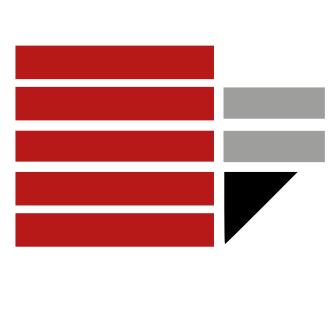
\includegraphics[height=1.30cm]{figures/unical_logo.png}}
		\end{center}
		
		\vspace{0.6cm}
		
		{\large\textsc{University of Calabria}\par}
		
		\vspace{0.25cm}
		
		{\LARGE\bfseries GroundEffect \par}
		
		\vspace{0.15cm}
		
		{\large A Formula One Data Warehouse for 2021--2022 Performance and Result Analysis\par}
		
		\vspace{0.35cm}
		
		{\large Design \& Data Management\par}
		
		\vspace{0.35cm}
		
		{\normalsize Rudi Giuseppe\par}
		\vspace{0.1cm}
		{\normalsize \today\par}
		
	\end{center}
	
	\vspace{0.4cm}
}

\begin{document}
	
	
	\customtitle
	

	\begin{abstract}
		Formula 1 data from the 2021 and 2022 seasons are used to build an analytical foundation for studying performance changes around the 2022 regulatory shift.
		Starting from API-based sources, the project defines a structured data pipeline that transforms raw racing data into a reconciled database and then into a multidimensional Data Warehouse. 
		The focus of this document is on the engineering and design choices made before the visualization stage: data re-engineering, data quality assessment, cleaning, fact schema design, and logical star schema construction.
	\end{abstract}

	\vspace{0.3cm}
	
	\noindent\textbf{Document scope.}
	The report highlights the most relevant decisions of the Formula 1 Data Warehouse pipeline.
	More detailed documentation for each stage is provided in ~\hyperref[sec:repository-material]{ Supplementary Material}.

	
	\tableofcontents
	\newpage
	

	\section{Project Goal}
	
	The project studies Formula 1 performance across the 2021 and 2022 seasons in order to understand how the regulatory change affected the competitive balance among teams. 
	This comparison is particularly meaningful because the 2022 season introduced a new technical framework, with a stronger emphasis on ground-effect aerodynamics leading to a substantial change in car design philosophy.
	
	Within this context, the goal of the project is to analyse how team performance changed across the two seasons and to observe how the new regulations influenced the balance of competitiveness. 
	The interest is therefore not only in absolute performance, but also in the relative changes that emerged across sessions, circuits, sectors, tyre conditions, and race contexts. This report focuses on the design and engineering choices, while the final visual exploration is developed separately in Tableau.
	
	
	\begin{figure}[H]
		\centering
		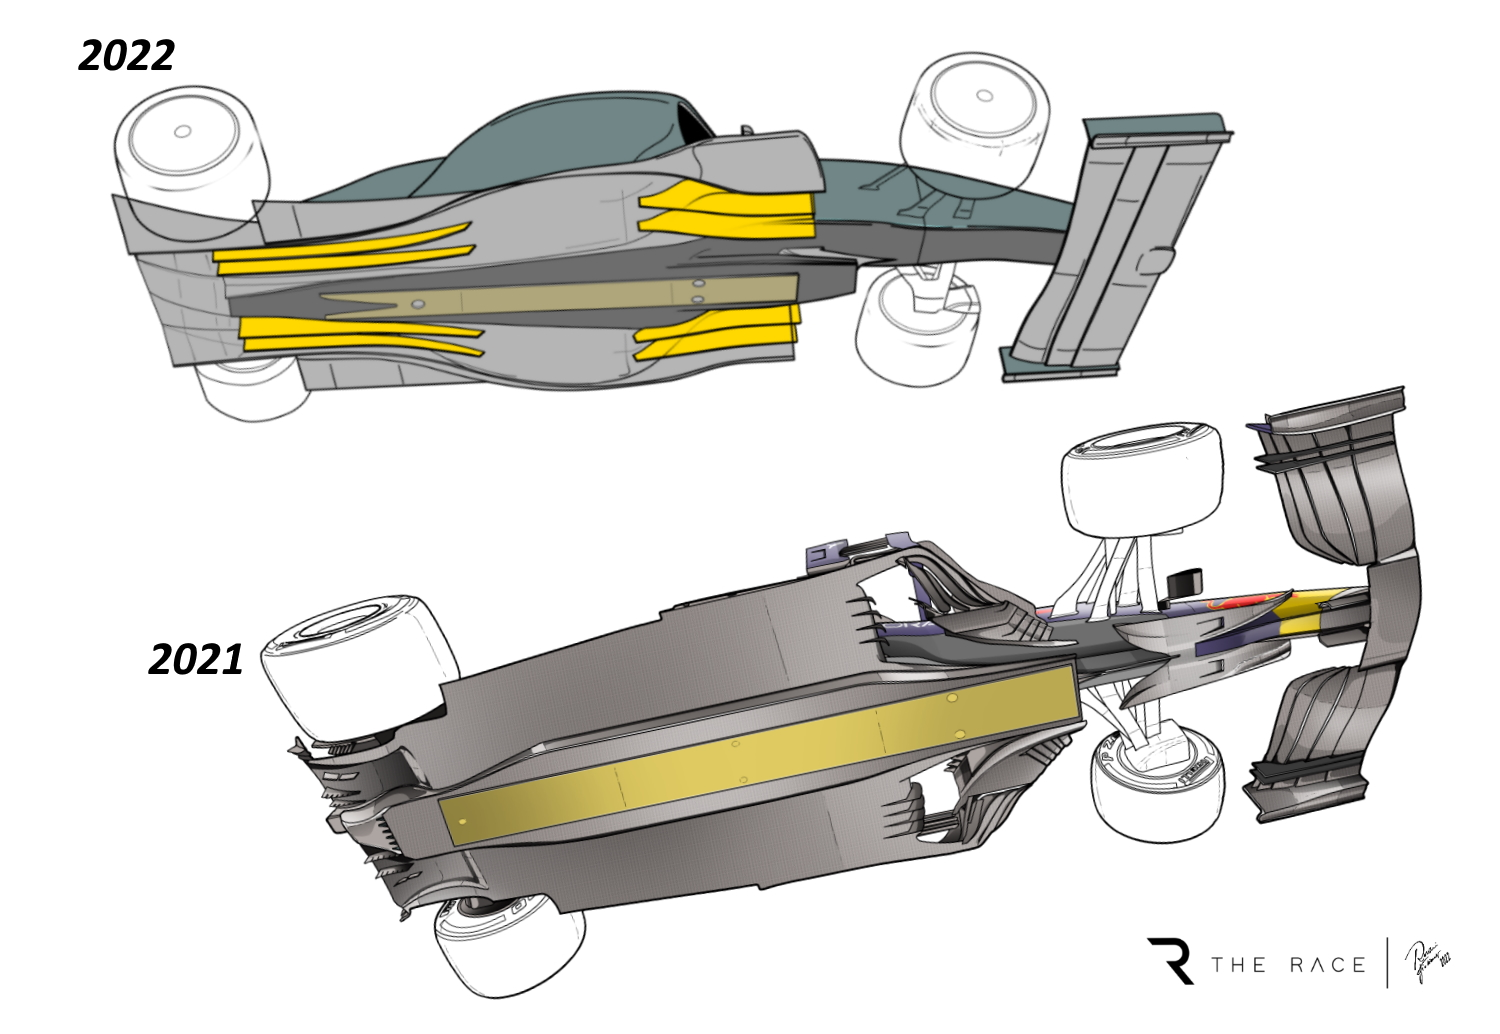
\includegraphics[width=0.50\linewidth]{figures/ground_effect.jpg}
		\caption{Conceptual representation of the 2022 regulatory change in car aerodynamics.}
		\label{fig:f1-regulation-change}
	\end{figure}

	
	
	\subsection{Business Questions}
	
	The general objective of the project can be expressed through the following main analytical question:
	
	\begin{quote}
		\textit{How did the 2022 regulatory change affect the competitive balance in Formula 1 between the 2021 and 2022 seasons?}
	\end{quote}
	
	This main question is then divided into more specific business questions. 
	Each of them focuses on a different analytical perspective, so that the final interpretation can be built by combining :
	
	\begin{itemize}
		\item Did the performance differences emerge more clearly in qualifying sessions or race sessions?
		\item How did performance vary according to tyre compound and tyre context?
		\item On which circuit types did the differences between teams become more visible?
		\item Did specific sector characteristics highlight different strengths or weaknesses of the cars?
	\end{itemize}

	
	
	\subsection{Project Roadmap}
	
	\begin{figure}[H]
		\centering
		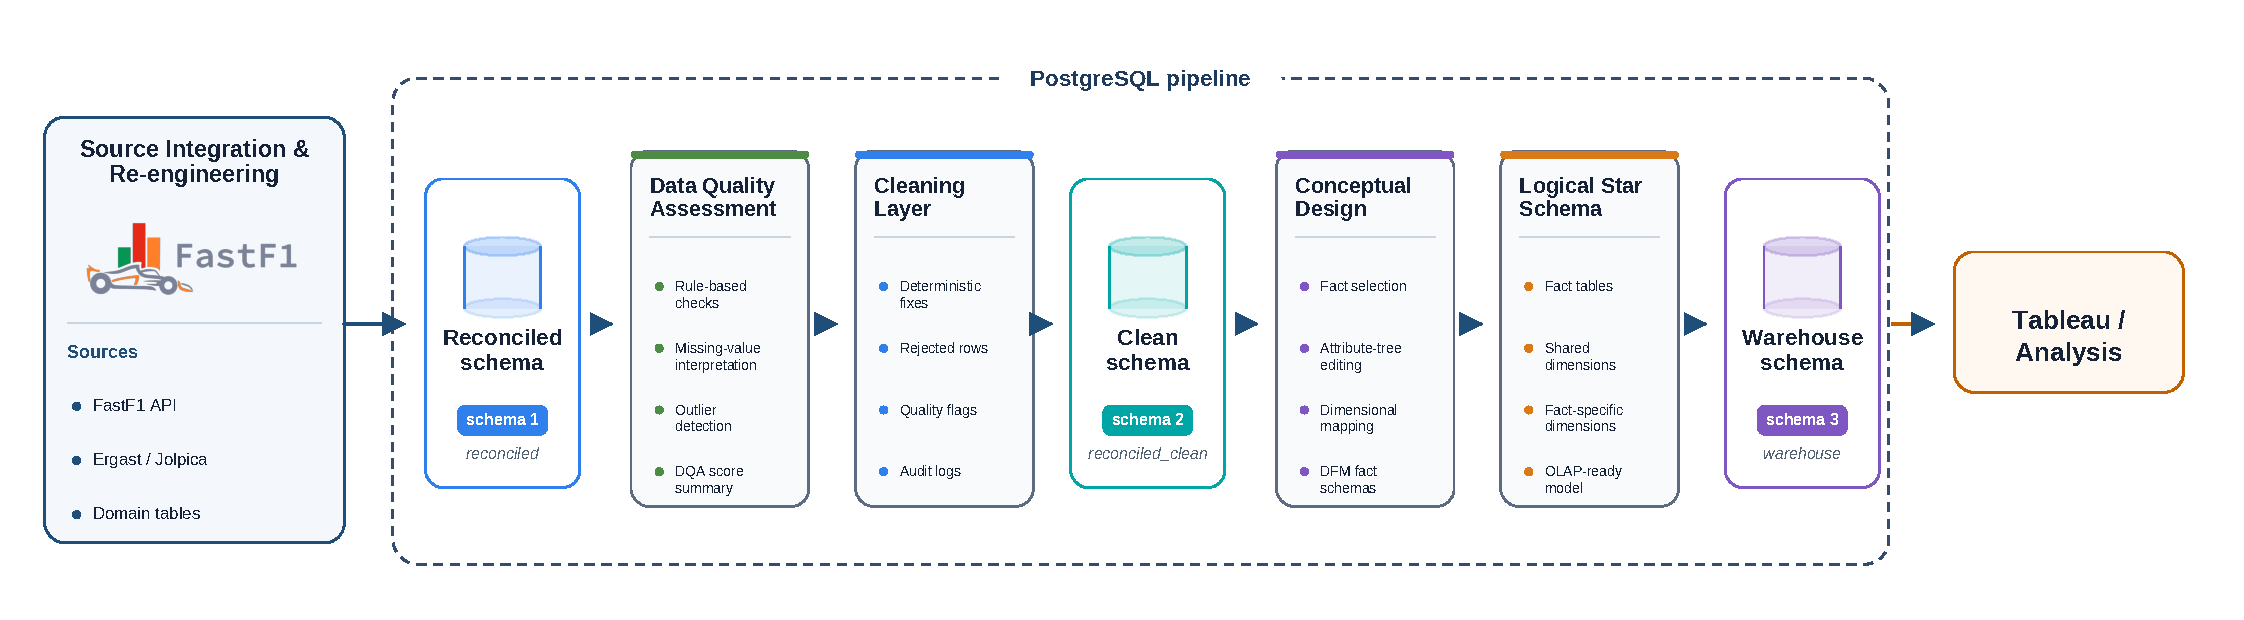
\includegraphics[width=1\linewidth]{figures/roadmap.pdf}
		\caption{Project-specific roadmap}
		\label{fig:project-roadmap}
	\end{figure}

	
	
	

	\section{Data Sources and Re-engineering}
	

	\subsection{Source Layer}
	
	The project mainly relies on API-based sources to extract structured Formula 1 data. 
	Additional analytical information was introduced through manually built domain tables, supported by domain knowledge and external descriptive sources. 
	The source layer is summarized in Table~\ref{tab:sources}.

	\begin{table}[H]
		\centering
		\caption{Source layer used in the project.}
		\label{tab:sources}
		\begin{tabularx}{\linewidth}{p{3.6cm}X}
			\toprule
			\textbf{Source} & \textbf{Information extracted} \\
			\toprule
			FastF1 API 
			& Event schedule, race weekends, Qualifying and Race sessions, session results, lap-level data, sector times, weather and track status. \\
			\midrule
			Ergast/Jolpica API 
			& Driver and constructor master data \\
			\midrule
		
			Domain knowledge 
			& Season-level information and circuit classification \\
			\bottomrule
		\end{tabularx}
	\end{table}

	

	\subsection{Re-engineering Strategy}
	
	The raw structures extracted from the APIs were not directly suitable for the construction of a reconciled relational database. 
	They were designed as API outputs and Python data structures, not as stable database relations for analytical use. 
	For this reason, the re-engineering phase transformed the extracted data into a coherent relational structure.
	
	Only the most relevant re-engineering decisions are reported in this section. 


	\subsubsection{Domain Tables}
	
	Two domain tables: \texttt{season} and \texttt{circuit} provide the season-level context and the circuit-level technical classification.
	Their attributes are shown in Figure~\ref{fig:domain-tables}, while the external sources used to populate and validate them are reported in the references~\cite{f1calendars,f1standings,formulaTimerCircuits}.

	
	\begin{figure}[H]
		\centering

		
\includegraphics[width=0.50\linewidth]{figures/domain_tables.pdf}
		\caption{Domain tables manually introduced.}
		\label{fig:domain-tables}
	\end{figure}
	

	\begin{table}[H]
		\centering
		\caption{Domain values for circuit and sector categories.}
		\label{tab:circuit-sector-categories}
		
		\begin{minipage}{0.46\linewidth}
			\centering
			\begin{tabularx}{\linewidth}{X}
				\toprule
				\textbf{\texttt{global\_circuit\_category}} \\
				\midrule
				\texttt{street} \\
				\texttt{power\_sensitive} \\
				\texttt{aero\_sensitive} \\
				\texttt{mixed} \\
				\bottomrule
			\end{tabularx}
		\end{minipage}
		\hfill
		\begin{minipage}{0.46\linewidth}
			\centering
			\begin{tabularx}{\linewidth}{X}
				\toprule
				\textbf{\texttt{sector*\_category}} \\
				\midrule
				\texttt{power} \\
				\texttt{fast\_corners} \\
				\texttt{slow\_corners} \\
				\texttt{technical} \\
				\bottomrule
			\end{tabularx}
		\end{minipage}
		
		\vspace{0.15cm}
		\footnotesize{\textit{Note:} \texttt{sector*\_category} refers to \texttt{sector1\_category}, \texttt{sector2\_category}, and \texttt{sector3\_category}.}
	\end{table}

	

	\subsubsection{Raw API Structures}
	
	Figure~\ref{fig:raw-api-overview} provides an aggregated overview of the raw structures obtained from the API-based sources. 
	The objective is to show that these information were not directly database-friendly. 
	The complete raw structures, including all original attributes, are reported in Appendix~\ref{appendix:raw-api-structures}.
	
	\begin{figure}[H]
		\centering

		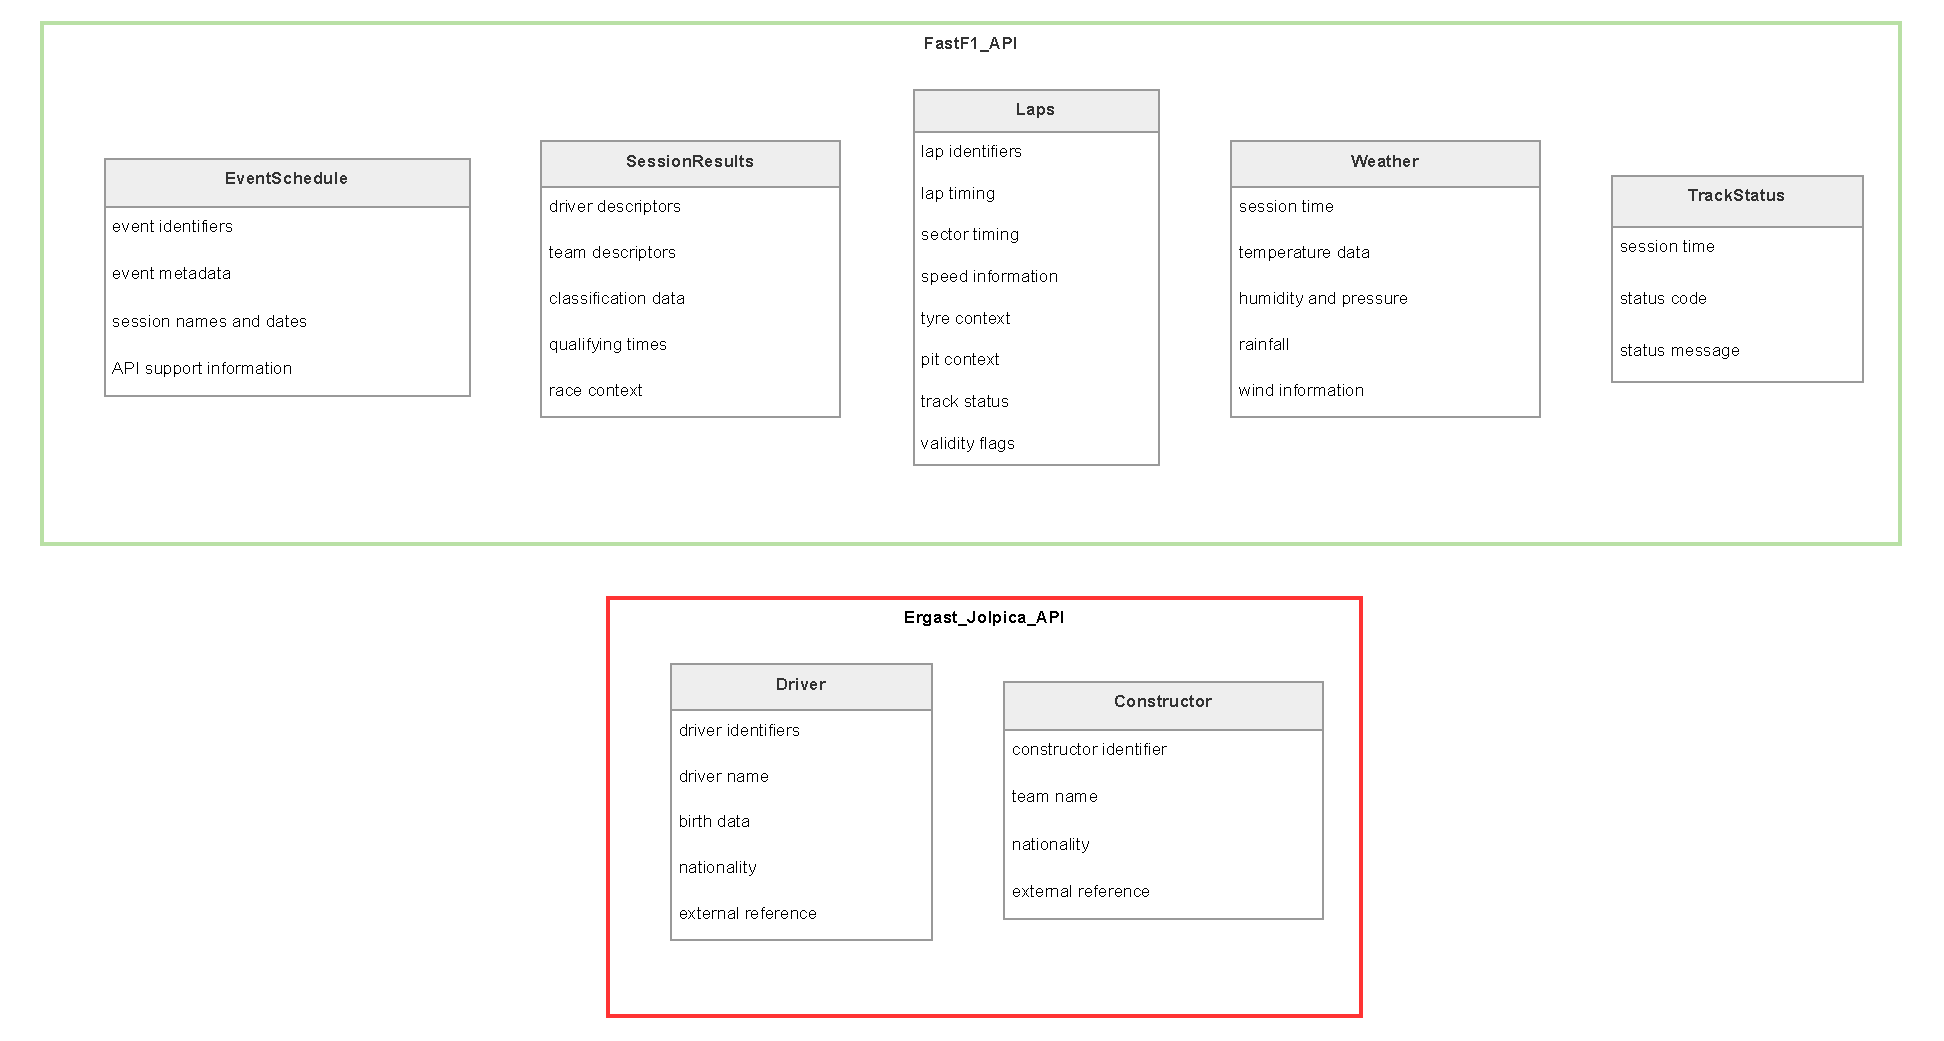
\includegraphics[width=0.95\linewidth]{figures/raw_tables_overview.pdf}
		\caption{Aggregated overview of the raw API structures.}
		\label{fig:raw-api-overview}
	\end{figure}

	
	
	
	\subsubsection{Main Re-engineering Decisions}
	

	The following paragraphs report the re-engineering decisions considered most relevant for understanding the transition from the raw API structures to the reconciled PostgreSQL schema. 
	
	After these main decisions, Table~\ref{tab:reengineering-summary} summarizes additional transformations.

	
	
	\paragraph{Analytical scope filtering.}

	Testing events were excluded because they are not part of the championship race calendar and do not follow the same round-based structure used for Grand Prix events. 
	Free practice sessions were also excluded because they are mainly used by teams for setup work, tyre evaluation, and race preparation. 
	Since the project focuses on comparable performance contexts, only Qualifying and Race sessions were retained.
	
	
	\paragraph{Separation of event-level and session-level information.}
	The raw event schedule returned by FastF1 contains both Grand Prix information and session-related information in the same structure. 
	This organization is not suitable for a relational schema because it mixes two different semantic levels. For this reason, the raw schedule was split into two relations: \texttt{grand\_prix} and \texttt{session}. 
	The \texttt{grand\_prix} table represents the event-level context of a race weekend, while the \texttt{session} table represents the lower-level sessions associated with that event. 
	This split makes the reconciled schema closer to the real Formula 1 structure: one season contains Grand Prix weekends, and each Grand Prix contains multiple sessions.
	

	\paragraph{Driver/team integration and redundancy control.}
	Driver and team identifiers were propagated into the performance-related tables, especially \texttt{lap} and \texttt{result}. 
	While \texttt{result} already provides the driver and team context at session level, raw lap data did not directly expose the official \texttt{driver\_id} and \texttt{team\_id}. 
	For this reason, lap records were enriched by matching them with the corresponding session result information. A separate \texttt{driver\_team\_season} association was also considered but not materialized. 
	The relationship can still be reconstructed through the existing links:
	
	\[
	\texttt{driver/team}
	\leftarrow
	\texttt{lap/result}
	\rightarrow
	\texttt{session}
	\rightarrow
	\texttt{grand\_prix}
	\rightarrow
	\texttt{season}
	\]
	
	Adding an explicit association table would therefore introduce redundancy without supporting the main analytical goal of the project, which focuses on performance analysis rather than driver-team career reconstruction.
	
	\begin{longtable}{p{4.2cm}p{\dimexpr\linewidth-4.2cm-4\tabcolsep\relax}}
		\caption{Additional re-engineering decisions.}
		\label{tab:reengineering-summary} \\
		
		\toprule
		\textbf{Decision} & \textbf{Motivation} \\
		\midrule
		\endfirsthead
		
		\toprule
		\textbf{Decision} & \textbf{Motivation} \\
		\midrule
		\endhead
		
		\bottomrule
		\endfoot
		
		Naming standardization 
		& API-oriented attribute names were converted from formats such as UpperCamelCase to \texttt{snake\_case} for a database-oriented naming convention. \\
		\midrule
		
		Surrogate PKs and FKs
		& Surrogate primary keys were introduced to provide stable row identifiers, while foreign keys were used to make table relationships explicit. \\
		\midrule
		
		Time conversion to \texttt{ms}
		& Time-related values returned by the APIs as timedelta were converted into integer milliseconds with the suffix \texttt{\_ms} to simplify numerical comparison. \\
		\midrule
		
		Removal of duplicated descriptors
		& Repeated driver, team, event, or session descriptors were removed when the same info could be recovered through joins with reference tables. \\
		
	\end{longtable}

	
	

	
	
	\subsubsection{Reconciled Database Overview}
	
	The output of the re-engineering phase is the reconciled PostgreSQL schema. 
	For readability, the E/R diagram in Figure~\ref{fig:reconciled-er-diagram} reports only the most relevant attributes. 
	
	The complete logical schema is reported in Appendix~\ref{appendix:logical-schema}.
	
	\vspace{2em}
	
	\begin{figure}[H]
		\centering
		 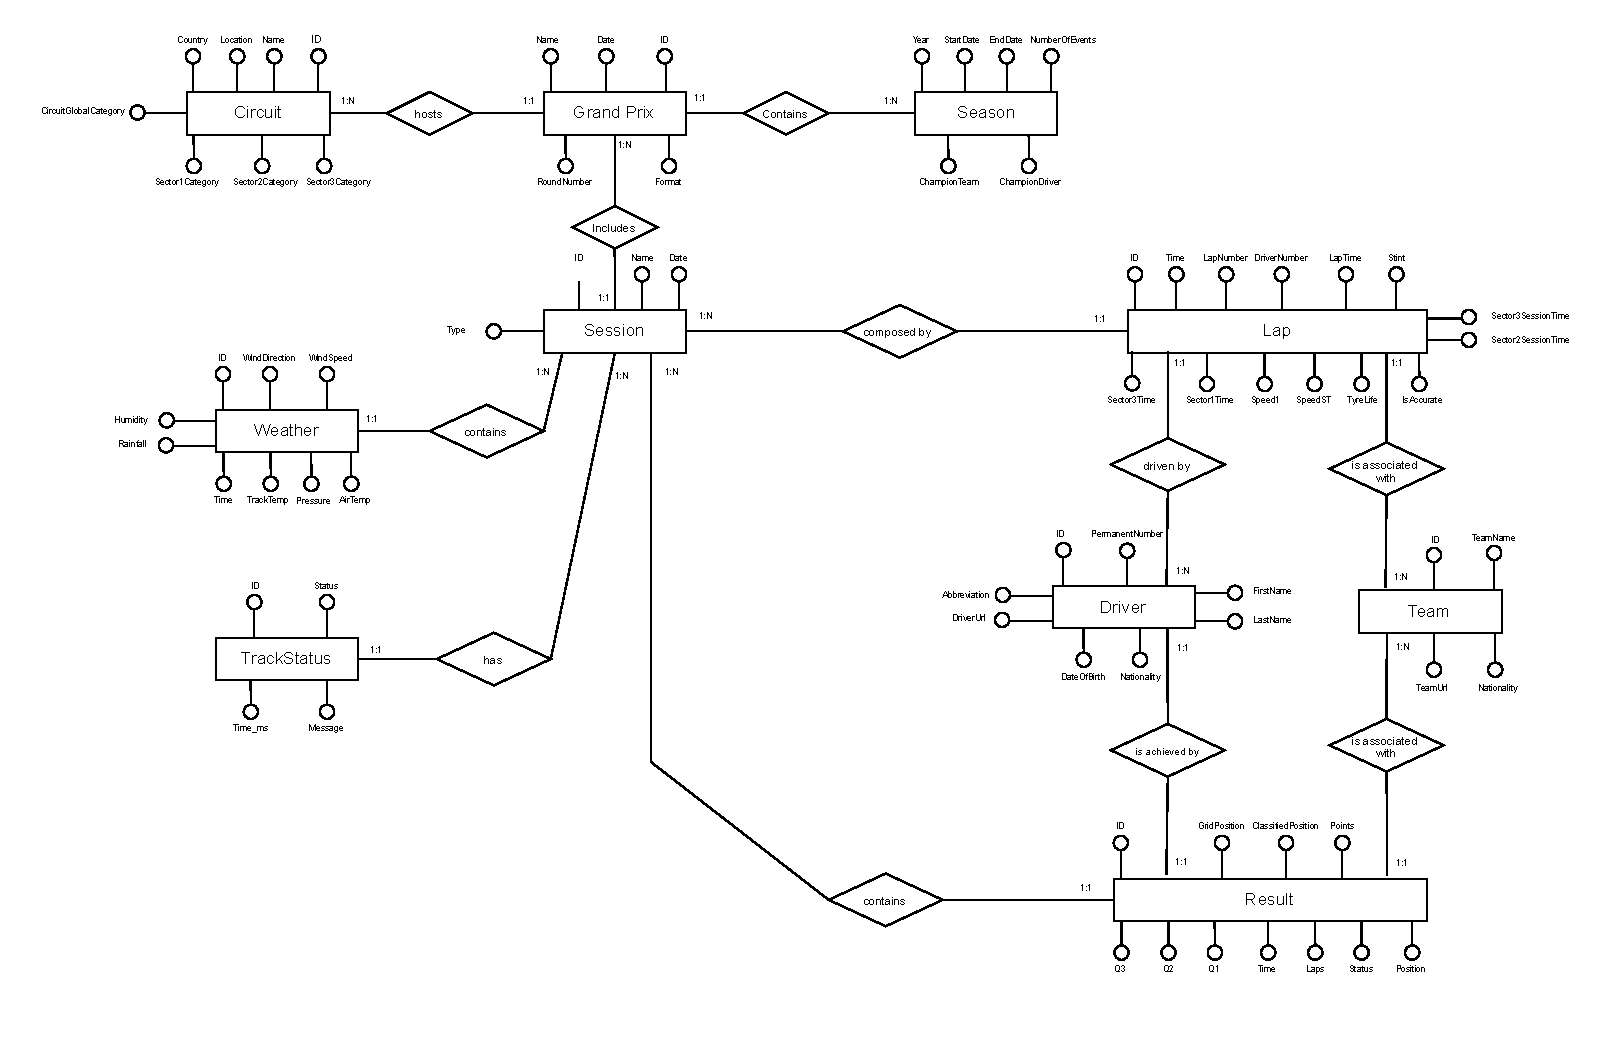
\includegraphics[width=1\linewidth]{figures/e-r.pdf}
		
		\caption{Simplified E/R diagram of the reconciled database}
		\label{fig:reconciled-er-diagram}
	\end{figure}

	

	\section{Data Quality Assessment}
	
	\subsection{Type Validation Scope}
	
	In a generic Data Quality Assessment workflow, type validation is an important preliminary step. The fact that a column is named as a date, a number, or a boolean attribute does not guarantee that its values actually follow the expected type.
	
	In this project, however, the source data are mainly obtained from API-based Python structures. Therefore, the input is not an uncontrolled textual source: each column already has an expected computational representation. For this reason, the Data Quality Assessment does not focus on generic type-parseability checks. Instead, it focuses on quality problems that can still exist after typed loading.
	
	\subsection{General Data Quality Assessment}
	
	The General Data Quality Assessment is applied to the reconciled schema in order to evaluate its structural and semantic quality, producing deterministic evidence for the following cleaning workflow without modifying the data.The assessment is organized according to the following data quality dimensions.
	
	\begin{table}[H]
		\centering
		\caption{DQA dimensions considered in the project.}
		\label{tab:dqa-dimensions}
		\renewcommand{\arraystretch}{1.35}
		\begin{tabularx}{0.85\linewidth}{
				>{\centering\arraybackslash}X
				>{\centering\arraybackslash}X
				>{\centering\arraybackslash}X
			}
			\toprule
			\textbf{Completeness} 
			& \textbf{Uniqueness} 
			& \textbf{Validity} \\
			
			\textbf{Consistency} 
			& \textbf{Accuracy} 
			& \textbf{Referential Integrity} \\
			\bottomrule
		\end{tabularx}
		
		\vspace{0.15cm}
		\footnotesize{\textit{Note:} Timeliness is excluded because the project uses historical seasons; temporal checks are treated as consistency rules.}
	\end{table}
	
	

	Since the complete set of rules is too detailed for the main report, this section presents only the most relevant assessment choices. A summarized dimension-by-dimension view is reported in Appendix~\ref{appendix:dqa-rules}.
	
	

	\begin{table}[H]
		\centering
		\small
		\caption{Representative Data Quality Assessment checks.}
		\label{tab:representative-dqa-checks}
		\begin{tabularx}{\linewidth}{p{5cm}X}
			\toprule
			\textbf{Representative check}
			& \textbf{Motivation} \\
			\midrule
			
			Lap timing coherence
			& Verifies that the sum of the three sector times is coherent with the total lap time, allowing a small tolerance for source precision. Pit-in and pit-out laps are excluded because they may distort normal lap-time interpretation. \\
			
			\midrule
			
			Race-weekend date coherence
			& Verifies that each Qualifying or Race session is temporally coherent with its Grand Prix. Sessions are expected to occur within the race weekend window, from two days before the Grand Prix date to the Grand Prix date. \\
			\midrule
			
			Track-status semantic coherence
			& Verifies that each numerical track-status code always corresponds to the expected textual message. For example, the same status code must always be associated with the same meaning, such as \texttt{1} with \texttt{AllClear}. \\
			
			\midrule
			
			Weather-context plausibility
			& Verifies that the difference between track temperature and air temperature remains within a broad plausible range. \\
			
			\midrule
			
			Circuit classification coverage
			& Verifies that circuit and sector classification attributes are present. \\
			
			\midrule
			
			Fact-grain uniqueness
			& A lap must be uniquely identified within a session-driver-lap-number combination, while a result must be unique for each driver in a session. \\
			
			\bottomrule
		\end{tabularx}
	\end{table}

	

	
	\subsection{Focused Missing Values Analysis}
	
	The focused missing-values analysis evaluates the analytical usability of the \texttt{lap} and \texttt{result} tables, which define the basis of the two Data Warehouse facts. In Formula 1 data, a null value is not always an error. Some null values are expected because of the sporting context or only in specific sessions or situations.
	For this reason, the missing-value script assigns two fields to each relevant null value: a missing class and a missing information area.
	
	
	\begin{table}[H]
		\centering
		\caption{Missing value classes used in the focused analysis.}
		\label{tab:missing-classes}
		\begin{tabularx}{0.85\linewidth}{p{4cm}X}
			\toprule
			\textbf{Missing class} & \textbf{Meaning} \\
			\midrule
			

			\texttt{EXPLAINED NULL}
			& The value is missing, but the missingness is explained by a Formula 1 domain rule. \\
			
			\midrule
			
			\texttt{SUSPICIOUS NULL}
			& The value is missing and no clear domain explanation is available. \\
			
			\bottomrule
		\end{tabularx}
	\end{table}
	
	The missing information area describes which type of analysis is affected by the missing value.
	A row may have issues in one or more areas, but it can still be used for analyses that do not depend on the affected information.
	The final interpretation of each missing value is obtained by combining the missing class and the missing information area.
	
	\begin{table}[!htbp]
		\centering
		\caption{Missing information areas for the \texttt{result} table.}
		\label{tab:result-missing-information-areas}
		\begin{tabularx}{0.85\linewidth}{p{3.6cm}X}
			\toprule
			\textbf{\texttt{result} area} & \textbf{Meaning} \\
			\midrule
			\texttt{CLASSIFICATION} & Final order or classification information. \\
			\texttt{QUALIFYING} & Qualifying-time information. \\
			\texttt{RACE CONTEXT} & Points, completed laps, status, or race time. \\
			\texttt{NONE} & No affected analytical area. \\
			\bottomrule
		\end{tabularx}
	\end{table}
	
	\begin{table}[H]
		\centering
		\caption{Missing information areas for the \texttt{lap} table.}
		\label{tab:lap-missing-information-areas}
		\begin{tabularx}{0.85\linewidth}{p{3.6cm}X}
			\toprule
			\textbf{\texttt{lap} area} & \textbf{Meaning} \\
			\midrule
			\texttt{LAP TIME} & Main lap-time information. \\
			\texttt{SECTOR} & One or more sector times. \\
			\texttt{SPEED} & Speed-trap information. \\
			\texttt{TYRE} & Compound or tyre-life information. \\
			\texttt{TRACK STATUS} & Track-condition context. \\
			\texttt{PIT} & Pit-related interpretation. \\
			\texttt{NONE} & No affected analytical area. \\
			\bottomrule
		\end{tabularx}
	\end{table}
	
	\paragraph{Missing values on the result table.}
	
	The \texttt{result} table includes both qualifying-related and race-related attributes, missing values are interpreted according to the session type.
	
	\begin{table}[H]
		\centering
		\caption{Session-dependent attributes in the \texttt{result} table.}
		\label{tab:result-session-dependent-attributes}
		\begin{tabularx}{0.85\linewidth}{
				>{\raggedright\arraybackslash}p{4.2cm}
				>{\raggedright\arraybackslash}X
			}
			\toprule
			\textbf{Attribute category}
			& \textbf{Attributes} \\
			\midrule
			
			Qualifying-related
			& \texttt{q1\_ms}, \texttt{q2\_ms}, \texttt{q3\_ms} \\
			
			\midrule
			
			Race-related
			& \texttt{classified\_position}, \texttt{status}, \texttt{points}, \texttt{laps}, \texttt{time\_ms} \\
			
			\bottomrule
		\end{tabularx}
	\end{table}
	
	In Race sessions, qualifying-related attributes are not applicable. 
	Therefore, missing values in the qualifying attributes are classified as \texttt{EXPLAINED NULL}, with \texttt{NONE} in missing information area. 
	By contrast, missing values in race-related attributes are classified as \texttt{SUSPICIOUS NULL}: missing position or classification information affects \texttt{CLASSIFICATION INFORMATION}, while missing race context values affect \texttt{RACE CONTEXT INFORMATION}.
	
	\vspace{1.5em}
	In Qualifying sessions, \texttt{position} is the control attribute used to interpret missing qualifying times. 
	If \texttt{position} is missing, qualifying progression cannot be reconstructed reliably; therefore, the value is classified as \texttt{SUSPICIOUS NULL} with \texttt{CLASSIFICATION INFORMATION}.
	
	The following rules identify the cases where a missing qualifying time is expected from the structure of the session.
	

	\begin{table}[H]
		\centering
		\small
		\caption{Expected nulls in Qualifying progression.}
		\label{tab:qualifying-expected-null-rules}
		\begin{tabularx}{0.95\linewidth}{
				>{\raggedright\arraybackslash}p{3.7cm}
				>{\raggedright\arraybackslash}p{3.1cm}
				>{\raggedright\arraybackslash}p{3cm}
				>{\raggedright\arraybackslash}X
			}
			\toprule
			\textbf{Condition}
			& \textbf{Missing attribute}
			& \textbf{Classification}
			& \textbf{Interpretation} \\
			\midrule
			
			\texttt{position > 15}
			& \texttt{q2\_ms}, \texttt{q3\_ms}
			& \texttt{EXPLAINED NULL} / \texttt{NONE}
			& The driver was eliminated in Q1. \\
			
			\midrule
			
			\texttt{11 <= position <= 15}
			& \texttt{q3\_ms}
			& \texttt{EXPLAINED NULL} / \texttt{NONE}
			& The driver was eliminated in Q2. \\
			
			\bottomrule
		\end{tabularx}
	\end{table}
	
	If a qualifying time is missing even though the driver's position indicates that the phase should normally have been reached, the value is classified as suspicious.
	

	
	Race-specific attributes in Qualifying sessions are not central to qualifying performance analysis and are therefore treated as \texttt{EXPLAINED NULL} when missing.
	
	\paragraph{Missing values on the lap table.}
	The main text focuses on pit-stop timestamps and \texttt{lap\_time\_ms}; detailed rules for sector times, speed values, tyre information, track status, and weather context are reported in Appendix~\ref{appendix:missing-rules}.
	
	\begin{table}[H]
		\centering
		\small
		\caption{Representative missing-value rules for the \texttt{lap} table.}
		\label{tab:lap-missing-value-main-rules}
		\begin{tabularx}{\linewidth}{
				>{\raggedright\arraybackslash}p{3.8cm}
				>{\raggedright\arraybackslash}p{3.2cm}
				>{\raggedright\arraybackslash}p{3.4cm}
				>{\raggedright\arraybackslash}X
			}
			\toprule
			\textbf{Condition}
			& \textbf{Missing attribute}
			& \textbf{Classification}
			& \textbf{Interpretation} \\
			\midrule
			
			The lap does not end with a pit entry.
			& pit\_in\_time\_ms
			& EXPLAINED NULL / NONE
			& Pit-in time is recorded only when the lap ends with a pit entry. \\
			
			\midrule
			
			The lap does not start from the pit lane.
			& pit\_out\_time\_ms
			& EXPLAINED NULL / NONE
			& Pit-out time is recorded only when the lap starts from the pit lane. \\
			
			\midrule
			
			No clear domain explanation is available.
			& lap\_time\_ms
			& SUSPICIOUS NULL / LAP TIME INFORMATION
			& The row lacks the main timing measure required for lap-level performance analysis. \\
			
			\bottomrule
		\end{tabularx}
	\end{table}

	\subsection{Focused Outlier Detection}
	
	Focused outlier detection is applied only to numerical attributes in the \texttt{lap} table. 

	
	\begin{table}[H]
		\centering
		\small
		\caption{Numerical lap-level attributes considered for outlier detection.}
		\label{tab:outlier-selected-attributes}
		\begin{tabularx}{0.85\linewidth}{
				>{\raggedright\arraybackslash}p{4.0cm}
				>{\raggedright\arraybackslash}X
			}
			\toprule
			\textbf{Attribute group}
			& \textbf{Selected attributes} \\
			\midrule
			
			Lap timing
			& lap\_time\_ms \\
			
			\midrule
			
			Sector timing
			& sector1\_time\_ms; sector2\_time\_ms; sector3\_time\_ms \\
			
			\midrule
			
			Speed values
			& speed\_i1; speed\_i2; speed\_fl; speed\_st \\
			
			\bottomrule
		\end{tabularx}
	\end{table}
	
	Outlier detection is applied only to a restricted subset of clean candidate laps within each session. 
	This choice reduces the risk of flagging values that are extreme only because of the race context, such as pit sequences, Safety Car periods, rain, traffic, or other abnormal conditions. 
	In these cases, a slow lap time or an unusual speed value may be statistically distant from the rest of the session, but it is not necessarily a data quality error.
	
	\vspace{1em}
	\noindent\textbf{Clean candidate conditions for outlier detection}
	
	\begin{multicols}{2}
		\begin{itemize}[leftmargin=*, noitemsep]
			\item \texttt{lap\_time\_ms} is present.
			\item \texttt{compound} is present.
			\item \texttt{pit\_in\_time\_ms} is null.
			\item \texttt{pit\_out\_time\_ms} is null.
			\item \texttt{track\_status = 1}, corresponding to \texttt{AllClear}.
			\item The corresponding session is classified as dry.
		\end{itemize}
	\end{multicols}
	
	A session is classified as dry only if all weather observations associated with that session have rainfall equal to false. 
	This conservative rule reduces the risk of comparing dry laps with laps affected by rain.
	
	The script applies two statistical methods: the IQR method and the Modified Z-score.
	
	\begin{table}[H]
		\centering
		\small
		\caption{Outlier detection methods used in the focused analysis.}
		\label{tab:outlier-methods}
		\begin{tabularx}{1\linewidth}{
				>{\raggedright\arraybackslash}p{3.6cm}
				>{\raggedright\arraybackslash}X
			}
			\toprule
			\textbf{Method}
			& \textbf{Rule} \\
			\midrule
			
			IQR method
			& $IQR = Q_3 - Q_1$; values outside $[Q_1 - 1.5 \cdot IQR,\; Q_3 + 1.5 \cdot IQR]$ are flagged. \\
			
			\midrule
			
			Modified Z-score
			& $M_i = \dfrac{0.6745(x_i - median(x))}{MAD}$; values with $|M_i| > 3.5$ are flagged. \\
			
			\bottomrule
		\end{tabularx}
	\end{table}
	
	For each checked value, the script assigns a consensus score from 0 to 2 according to how many methods flag the value. 

	
	\subsection{Visual Summary of Data Quality Outputs}
	
	The Data Quality Assessment phase also produced visual outputs to summarize the evidence generated by the scripts. 

	
	\begin{figure}[H]
		\centering
		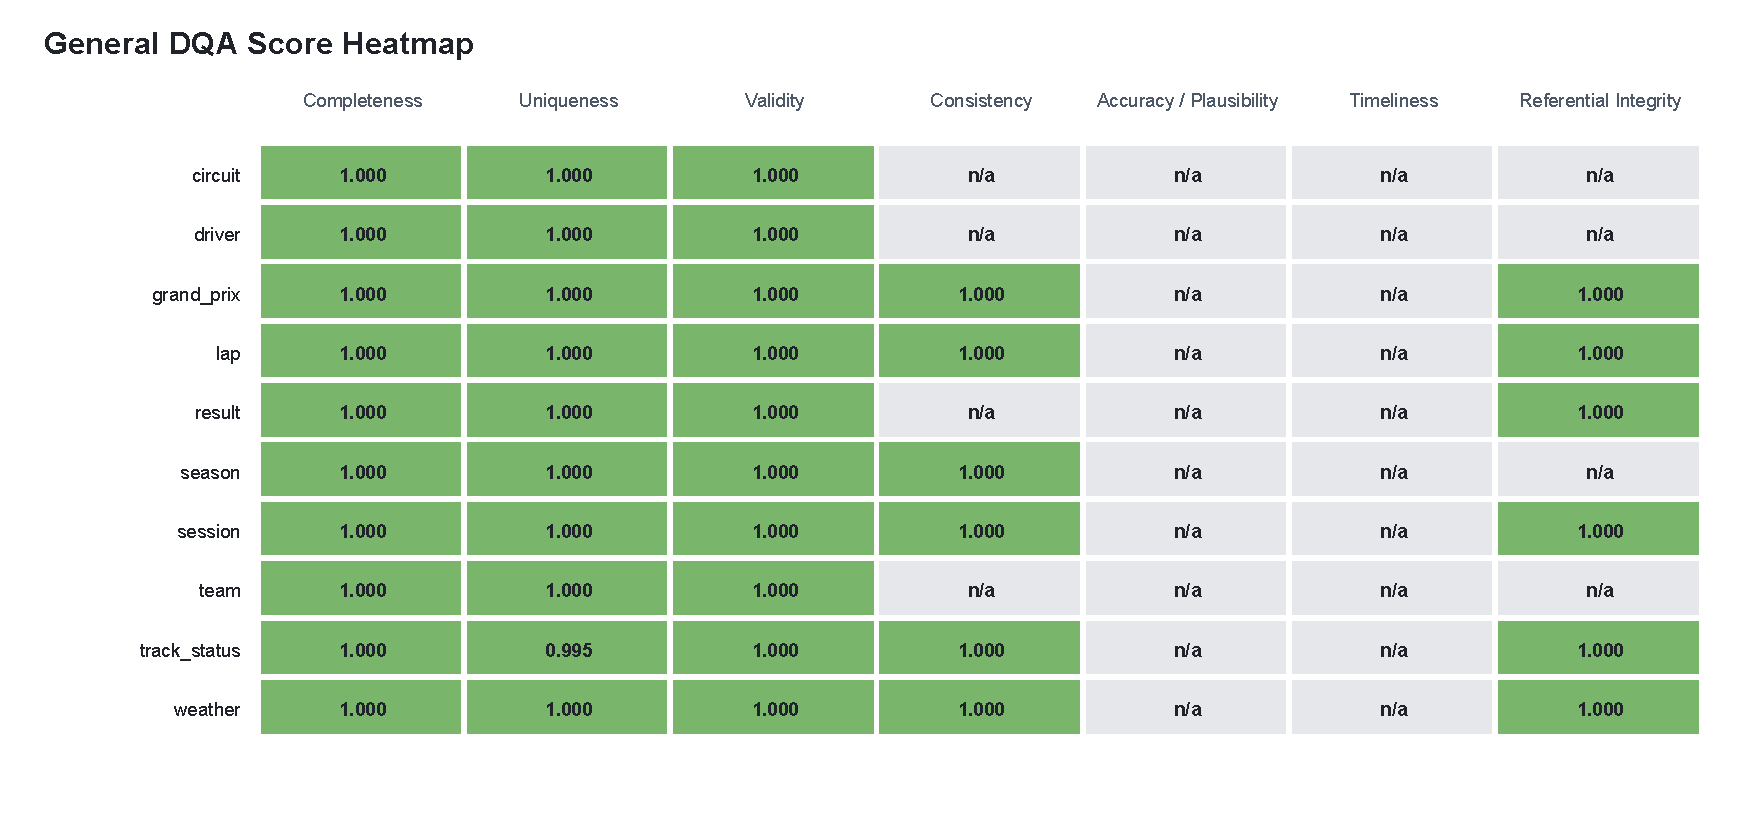
\includegraphics[width=1\linewidth]{figures/dqa_dimension_heatmap.pdf}
		\caption{General Data Quality Assessment score heatmap.}
		\label{fig:dqa-dimension-heatmap}
	\end{figure}
	
	The heatmap shows that the general DQA scores are very high across almost all tables and quality dimensions. 
	This result should not be interpreted as the absence of data quality problems. 
	The general assessment was intentionally based on deterministic and structural checks.More domain-specific issues, especially missing values and numerical anomalies, are analysed separately through the focused missing-value interpretation and outlier detection procedures.
	
	\begin{figure}[H]
		\centering
		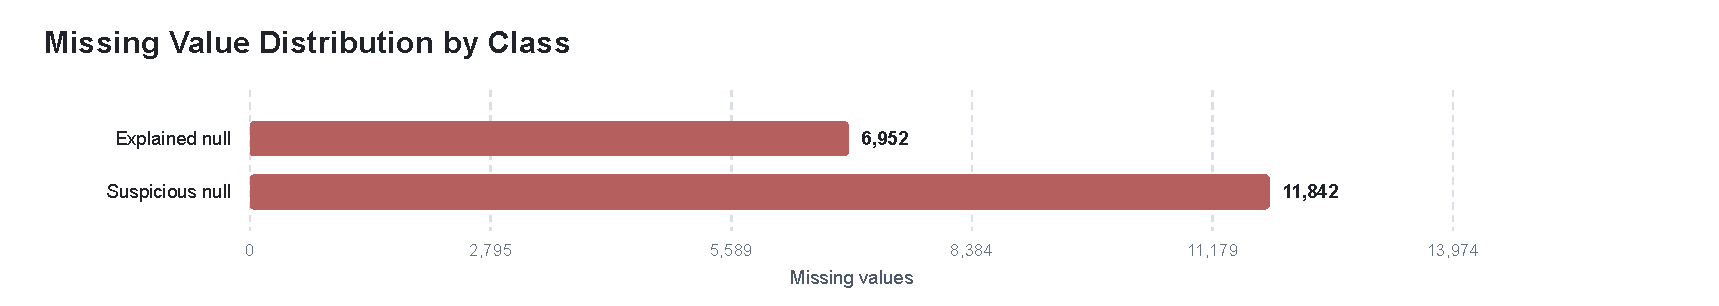
\includegraphics[width=0.90\linewidth]{figures/missing_class_distribution.pdf}
		\caption{Missing-value class distribution.}
		\label{fig:missing-class-distribution}
	\end{figure}
	
	\begin{figure}[H]
		\centering
		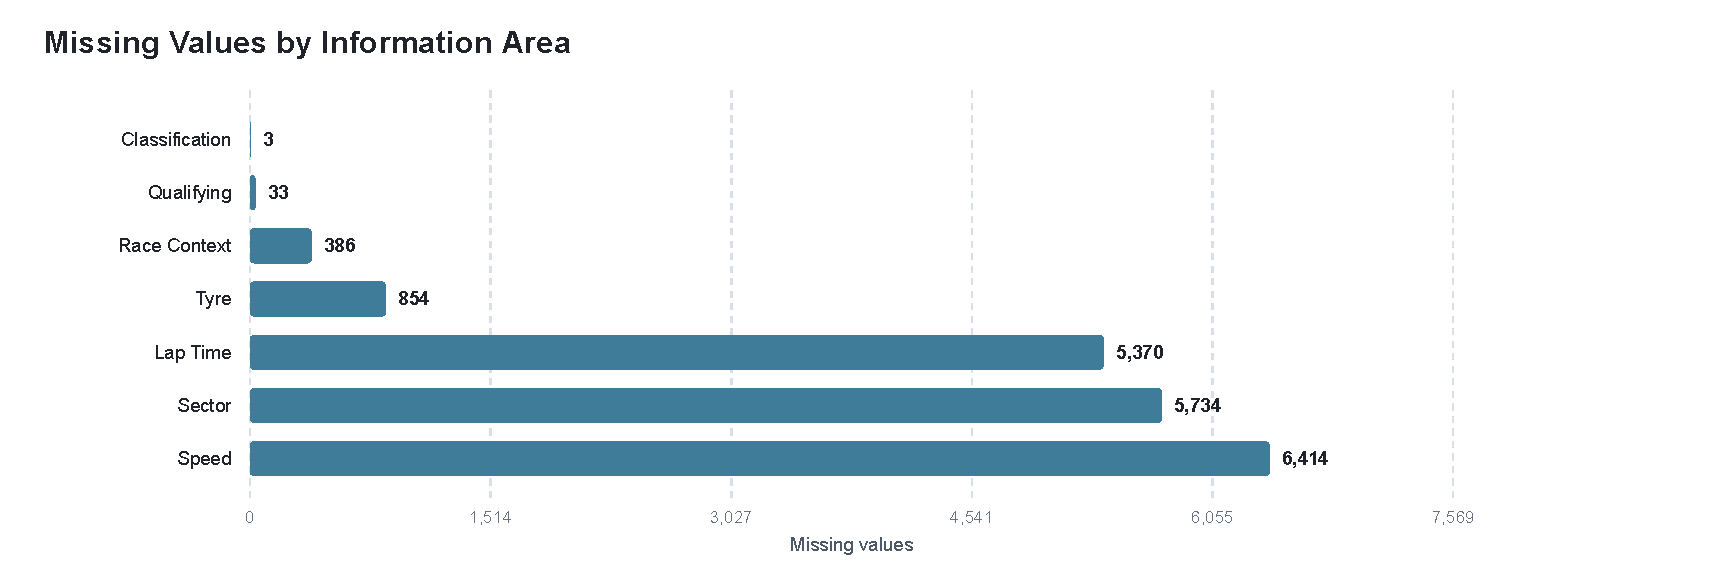
\includegraphics[width=0.90\linewidth]{figures/missing_information_area.pdf}
		\caption{Missing values by information area.}
		\label{fig:missing-information-area}
	\end{figure}
	
	The missing-value plots show that a relevant part of the null values is explained by the Formula One domain. The distribution by information area shows that missing values are mainly concentrated in speed, sector, and lap-time information. 
	This is coherent with the structure of lap-level data: sector times are collected across three circuit sectors, while speed values can be recorded at multiple detection points within the same lap. 
	Since these measurements are more granular, they also have more opportunities to contain incomplete information.
	
	\begin{figure}[H]
		\centering
		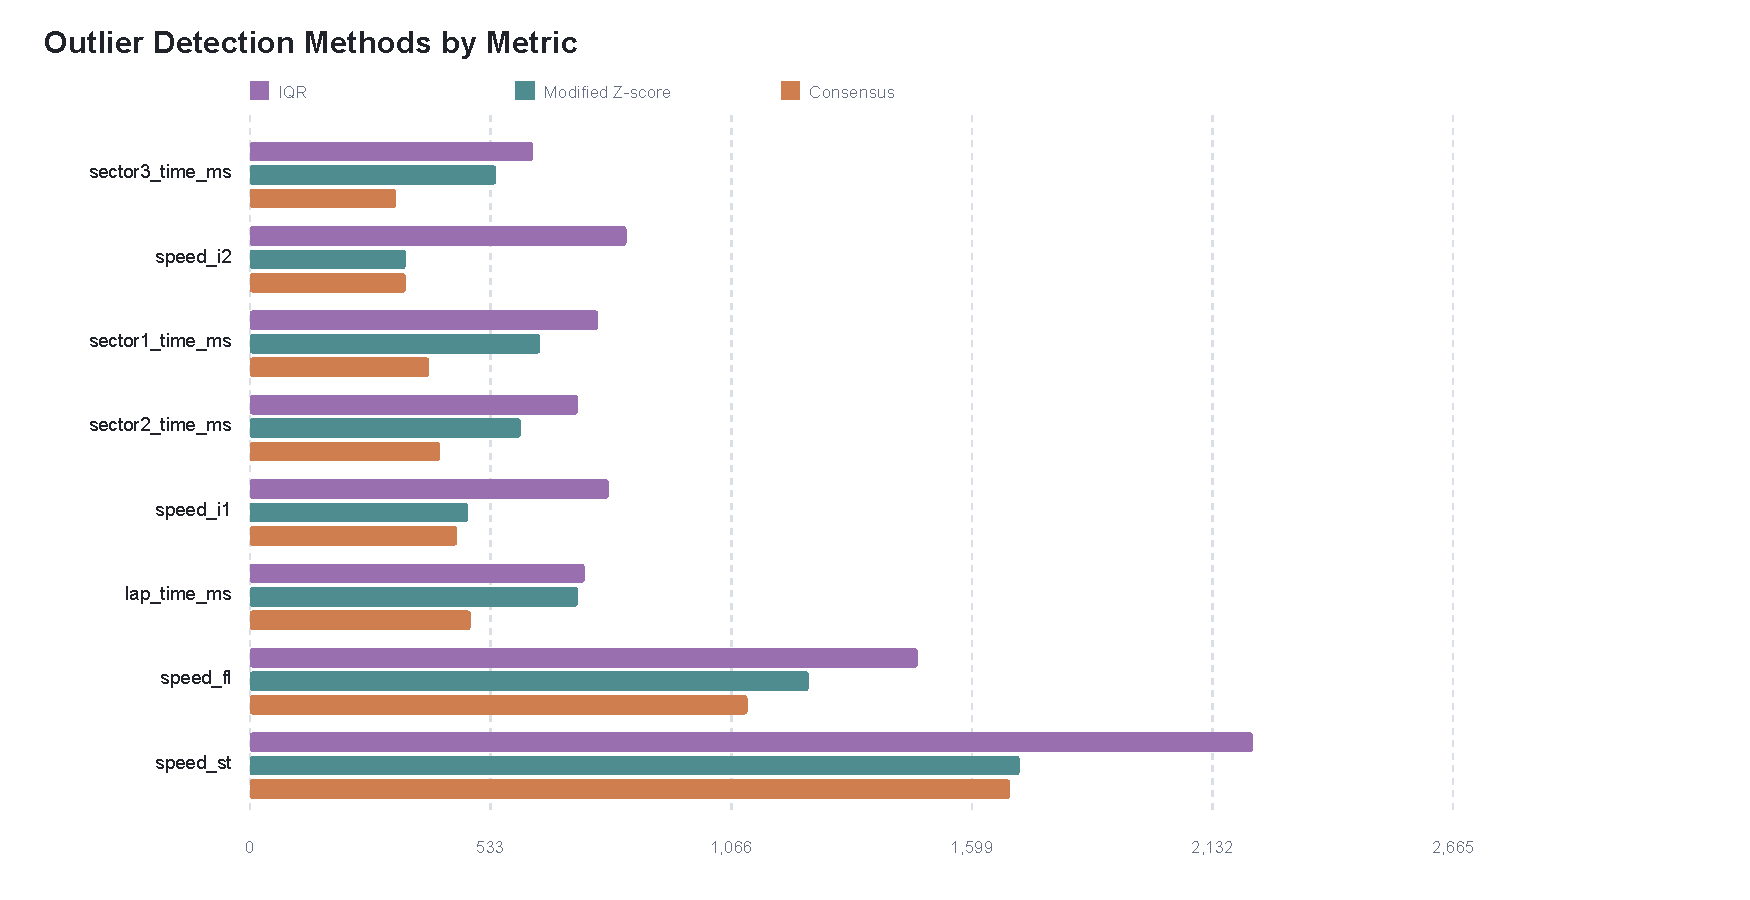
\includegraphics[width=1\linewidth]{figures/outlier_methods_by_metric.pdf}
		\caption{Outlier detection methods by metric.}
		\label{fig:outlier-methods-by-metric}
	\end{figure}
	
	
	The outlier-method comparison shows that the consensus rule reduces the number of values treated as strong anomalies. 
	Compared with the individual methods, especially the IQR method.
	
	\subsection{LLM-supported Interpretation}
	
	After the visual summaries, the artefacts produced by the Data Quality Assessment phase were also provided to a Large Language Model to support the interpretation of the detected issues. 

	The LLM was not used to modify the data or to make automatic cleaning decisions. 
	Its role was limited to producing a structured textual interpretation of the quality evidence. 
	In particular, three outputs were generated: a natural-language stakeholder summary, a more technical summary for developers and analysts, and a list of suggested cleaning priorities.

	The prompt provided to the LLM, together with an example of the generated output, is reported in Appendix~\ref{appendix:llm-dqa-interpretation}.

	\section{Data Cleaning}
	
	The Data Cleaning phase uses the evidence produced by the previous Data Quality Assessment section. 
	Unlike that phase, this step produces a new cleaned analytical layer derived from the reconciled database.
	
	The cleaning process follows a conservative approach using the following action types : 
	
	\begin{table}[H]
		\centering
		\small
		\caption{Cleaning actions.}
		\label{tab:cleaning-actions}
		\begin{tabularx}{0.95\linewidth}{
				>{\raggedright\arraybackslash}p{3.2cm}
				>{\raggedright\arraybackslash}X
			}
			\toprule
			\textbf{Action}
			& \textbf{Meaning} \\
			\midrule
			
			STANDARDIZE
			& Convert a value into a deterministic standard representation. \\
			
			\midrule
			
			SET NULL
			& Remove an invalid or unreliable value while preserving the row. \\
			
			\midrule
			
			DROP ROW
			& Remove a row that cannot preserve core analytical meaning. \\
			
			\midrule
			
			ADD FLAG
			& Preserve the row and mark the affected analytical area through a quality flag. \\
			
			\bottomrule
		\end{tabularx}
	\end{table}
	
	
	Before applying issue-specific policies, two common cleaning rules are applied to textual attributes. 
	
	\begin{table}[H]
		\centering
		\caption{General cleaning rules applied before issue-specific policies.}
		\label{tab:general-cleaning-rules}
		\begin{tabularx}{\linewidth}{p{2.7cm}p{9cm}X}
			\toprule
			\textbf{Rule} & \textbf{Condition} & \textbf{Action} \\
			\midrule
			\texttt{CR\_COMMON\_1} 
			& Textual values contain leading or trailing spaces. 
			& \texttt{STANDARDIZE} \\
			\midrule
			\texttt{CR\_COMMON\_2} 
			& Empty strings remain after trimming. 
			& \texttt{SET NULL} \\
			\bottomrule
		\end{tabularx}
	\end{table}
	
	\subsection{Cleaning Policies from General DQA}
	
	Only the most representative policies are reported. The complete DQA-driven cleaning rules are reported in Appendix~\ref{appendix:dqa-cleaning-rules}.
	
	
	\begin{table}[H]
		\centering
		\small
		\caption{Representative cleaning policies driven by General DQA.}
		\label{tab:dqa-cleaning-examples}
		\begin{tabular}{
				>{\centering\arraybackslash}m{2cm}
				>{\raggedright\arraybackslash}m{9.1cm}
				>{\raggedright\arraybackslash}m{5cm}
			}
			\toprule
			\textbf{Table}
			& \textbf{DQA issue}
			& \textbf{Cleaning action} \\
			\midrule
			
			lap
			& Missing structural identifiers, invalid lap number, or invalid lap time.
			& DROP ROW \\
			
			\midrule
			
			lap
			& Invalid sector, speed, or tyre-context values.
			& SET NULL + ADD FLAG 
			{\scriptsize
				(has\_sector\_information\_issue, 
				has\_speed\_information\_issue, 
				has\_tyre\_information\_issue)} \\
			
			\midrule
			
			result
			& Missing structural identifiers or invalid position.
			& DROP ROW \\
			
			\midrule
			
			result
			& Invalid points, completed laps, race time, or grid position.
			& SET NULL \\
			
			\midrule
			
			circuit
			& Invalid global or sector category.
			& STANDARDIZE / DROP ROW \\
			
			\midrule
			
			track\_status
			& Invalid status message, unknown status code, or code-message mismatch.
			& STANDARDIZE / DROP ROW \\
			
			\bottomrule
		\end{tabular}
	\end{table}
	
	\subsection{Cleaning Policies from Missing Values}
	
		\begin{table}[H]
		\centering
		\small
		\caption{Missing-value-driven cleaning policies for the \texttt{result} table.}
		\label{tab:result-missing-cleaning}
		\begin{tabularx}{\linewidth}{
				>{\raggedright\arraybackslash}m{6cm}
				>{\raggedright\arraybackslash}m{4.2cm}
				>{\raggedright\arraybackslash}X
			}
			\toprule
			\textbf{Missing information area}
			& \textbf{Cleaning action}
			& \textbf{Effect} \\
			\midrule
			
			CLASSIFICATION INFORMATION
			& DROP ROW
			& { \scriptsize Row removed} \\
			
			\midrule
			
			QUALIFYING INFORMATION
			& ADD FLAG
			& {\scriptsize has\_qualifying\_information\_issue = true} \\
			
			\midrule
			
			RACE CONTEXT INFORMATION
			& ADD FLAG
			& {\scriptsize has\_race\_context\_information\_issue = true}  \\
			
			\bottomrule
		\end{tabularx}
	\end{table}
	
	
	\begin{table}[H]
		\centering
		\small
		\caption{Missing-value-driven cleaning policies for the \texttt{lap} table.}
		\label{tab:lap-missing-cleaning}
		\begin{tabularx}{\linewidth}{
				>{\raggedright\arraybackslash}m{6cm}
				>{\raggedright\arraybackslash}m{4.2cm}
				>{\raggedright\arraybackslash}X
			}
			\toprule
			\textbf{Missing information area}
			& \textbf{Cleaning action}
			& \textbf{Effect} \\
			\midrule
			
			LAP TIME INFORMATION
			& DROP ROW
			& { \scriptsize Row removed} \\
			
			\midrule
			
			SECTOR INFORMATION
			& ADD FLAG
			& {\scriptsize has\_sector\_information\_issue = true} \\
			
			\midrule
			
			SPEED INFORMATION
			& ADD FLAG
			& {\scriptsize has\_speed\_information\_issue = true}  \\
			
			\midrule
			
			TYRE INFORMATION
			& ADD FLAG
			& {\scriptsize has\_tyre\_information\_issue = true} \\
			
			\midrule
			
			WEATHER INFORMATION
			& ADD FLAG
			& {\scriptsize has\_weather\_information\_issue = true} \\
			
			\midrule
			
			TRACK STATUS INFORMATION
			& ADD FLAG
			& {\scriptsize has\_track\_status\_information\_issue = true} \\
			
			\midrule
			
			PIT INFORMATION
			& ADD FLAG
			& {\scriptsize has\_pit\_information\_issue = true}  \\
			
			\bottomrule
		\end{tabularx}
	\end{table}
	
	\subsection{Cleaning Policies from Outlier Detection}
	
	
	\begin{table}[H]
		\centering
		\small
		\caption{Outlier-driven cleaning policies for the \texttt{lap} table.}
		\label{tab:outlier-cleaning}
		\begin{tabularx}{\linewidth}{
				>{\raggedright\arraybackslash}m{3.8cm}
				>{\centering\arraybackslash}m{3.0cm}
				>{\raggedright\arraybackslash}m{3.8cm}
				>{\raggedright\arraybackslash}X
			}
			\toprule
			\textbf{Metric}
			& \textbf{Consensus score}
			& \textbf{Cleaning action}
			& \textbf{Effect} \\
			\midrule
			
			lap\_time\_ms
			& 2
			& DROP ROW
			& { \scriptsize Row removed} \\
			
			\midrule
			
			lap\_time\_ms
			& 1
			& No cleaning action
			& { \scriptsize Row preserved} \\
			
			\midrule
			
			Sector time metrics
			& 1 or 2
			& ADD FLAG
			& {\scriptsize has\_sector\_information\_issue = true}  \\
			
			\midrule
			
			Speed metrics
			& 1 or 2
			& ADD FLAG
			& {\scriptsize has\_speed\_information\_issue = true} \\
			
			\bottomrule
		\end{tabularx}
	\end{table}
	
	This policy preserves as much information as possible. 
	For example, a lap with a suspicious speed value can still be used for lap-time analysis, but it should be excluded from speed-based analysis by filtering out rows where {\scriptsize has\_speed\_information\_issue = true}.
	
	\section{Conceptual Design of the Fact Schemas}
	
	The conceptual design phase moves from the reconciled relational schema to the analytical structure of the Data Warehouse. To support the analytical goal of the project, two complementary perspectives are required and are reported in Table~\ref{tab:facts-grain}.
	
	\begin{table}[H]
		\centering
		\small
		\caption{Selected facts and analytical grain.}
		\label{tab:facts-grain}
		\begin{tabularx}{\linewidth}{
				>{\raggedright\arraybackslash}p{3.3cm}
				>{\raggedright\arraybackslash}X
				>{\raggedright\arraybackslash}X
			}
			\toprule
			\textbf{Fact}
			& \textbf{Grain}
			& \textbf{Analytical focus} \\
			\midrule
			
			Lap Performance
			& One lap performed by one driver in one specific session, Grand Prix, and season.
			& Lap time, sector times, speed values, tyres, circuit characteristics, weather context, and track status. \\
			
			\midrule
			
			Session Result
			& One driver result in one specific session, Grand Prix, and season.
			& Qualifying outcomes, race outcomes, classification, points, and race completion. \\
			
			\bottomrule
		\end{tabularx}
	\end{table}
	
	\subsection{Attribute Tree Construction and Editing Strategy}
	
	Starting from the two selected facts, two attribute trees were built. Although the two facts have different grains, many branches are shared because both facts describe events that occur within the same Formula 1 context. 
	For this reason, the shared branches are first identified as follows:
	
	\begin{center}
		\begin{minipage}{0.75\linewidth}
			\begin{multicols}{3}
				\begin{itemize}[leftmargin=*, noitemsep]
					\item Driver
					\item Team
					\item Session
					\item Grand Prix
					\item Circuit
					\item Season
				\end{itemize}
			\end{multicols}
		\end{minipage}
	\end{center}
	
	
	Before presenting the attribute-tree editing diagrams, a common color legend is introduced. 
	The same colors are used in all diagrams to distinguish the operations applied to the nodes.
	
	\begin{table}[H]
		\centering
		\small
		\caption{Color legend for attribute-tree editing diagrams.}
		\label{tab:attribute-tree-editing-legend}
		\setlength{\tabcolsep}{8pt}
		\begin{tabular}{@{}c l | c l | c l@{}}
			\toprule
			\legendbox{pruninggreen} & Pruning
			& \legendbox{graftingred} & Grafting
			& \legendbox{derivedblue} & Derived attribute \\
			\bottomrule
		\end{tabular}
	\end{table}
	\subsubsection{Shared-Branch Editing Decisions}
	
	Since the shared branches will become common dimensions in the logical schema, they are edited with a single strategy valid for both facts. 
	Attributes that are useful for at least one fact are retained in the shared branch.
	

	\medskip
	\noindent\textbf{Race-weekend branch: Session, Grand Prix, Circuit, and Season.}
	\par\smallskip
	
	\begin{figure}[H]
		\centering
		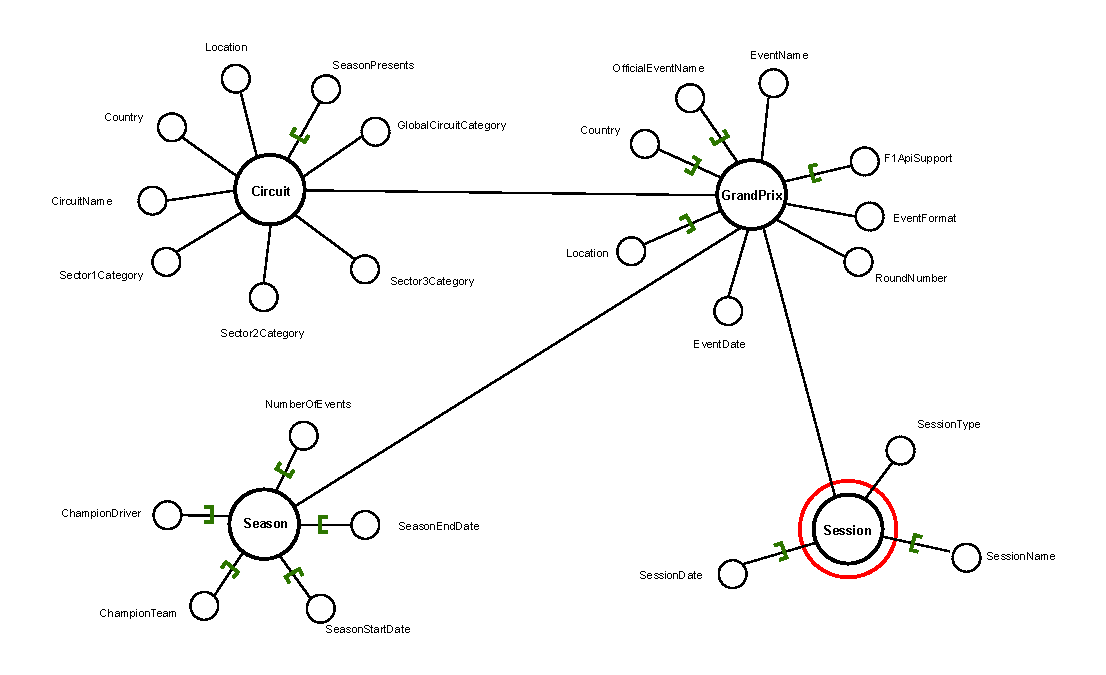
\includegraphics[width=1\linewidth]{figures/season-grandprix-session.pdf}
		\caption{Editing decisions for the shared race-weekend branches.}
		\label{fig:shared-race-weekend-editing}
	\end{figure}
	 
	For the \texttt{circuit} node, \texttt{seasons\_present} is pruned because it is descriptive coverage metadata.
	
	\medskip
	
	For the \texttt{grand\_prix} node, \texttt{official\_event\_name} is pruned because the shorter \texttt{event\_name} already provides a readable analytical label. The attributes \texttt{country} and \texttt{location} are also pruned from \texttt{grand\_prix} because the same geographical context is represented through the linked \texttt{circuit} branch. Finally, \texttt{f1\_api\_support} is pruned because it is a source-support flag.
	
	\medskip
	
	For the \texttt{season} node,all the attribute are pruned because they are contextual attributes that are not needed as aggregation levels. After this pruning, the season branch is reduced to \texttt{season\_year} directly associated with the \texttt{grand\_prix} branch.
	
	\medskip
	
	For the \texttt{session} node, \texttt{session\_date} and \texttt{session\_name} are pruned because the analysis only requires the session type. 
	The \texttt{session\_id} node is then grafted: the technical identifier is removed and as a result, \texttt{session\_type} becomes directly connected to the fact root, either \textit{Lap Performance} or \textit{Session Result}.
	
	\vspace{7em}
	\noindent\textbf{Participant branch: Driver and Team.}
	\par\smallskip
	
	\begin{figure}[H]
		\centering
		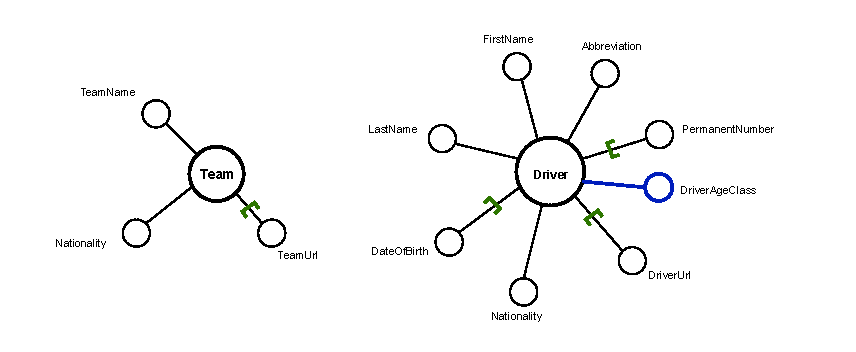
\includegraphics[width=1\linewidth]{figures/driver-team.pdf}
		
		\caption{Editing decisions for the shared Driver and Team branches.}
		\label{fig:shared-driver-team-editing}
	\end{figure}
	
	
	For the Driver branch, permanent number are pruned because they are not analytically significant. 
	The raw date of birth is not retained as an analytical level, but it is used to derive \texttt{driver\_age\_class}, a categorical attribute that can assume three values:
	\vspace{0.5em}
	
	\quad $\bullet$ Young 
	\quad $\bullet$ Intermediate 
	\quad $\bullet$ Senior.
	
	\vspace{0.5em}
	
	Team and Driver URL is pruned because it is only an external reference. 
	Nationality attributes are retained in both the Driver and Team branches, although they are more relevant for result-oriented analysis than for detailed lap-performance analysis.
	
	
	\subsubsection{Treatment of Time-dependent Context}
	
	The \texttt{weather} and \texttt{track\_status} tables require a separate treatment because they are not static descriptors of a session. 
	Both tables contain the attribute \texttt{time\_ms}, which identifies the time instant within the session at which the observation or status change is recorded.
	
	For this reason, a single session can be associated with multiple weather observations and multiple track-status records. 
	Therefore, these tables cannot be inserted as normal static branches of the attribute tree: their values are not determined only by the session, but also by the time instant inside the session.
	
	Instead, their information is transformed into derived contextual attributes, defined according to the grain of each fact. 
	For the \textit{Lap Performance} fact, the time-dependent context is aligned with each lap, while for the \textit{Session Result} fact it is summarized at session level when useful for result interpretation.
	
	\subsection{Fact-specific Attribute Tree Editing}
	
	After the shared branches have been edited, the remaining decisions concern the attributes that are specific to each fact root. 

	
	\subsubsection{Lap Performance Editing}
	
	The \textit{Lap Performance} fact is rooted in the \texttt{lap} relation. Table~\ref{tab:lap-pruning-representative} reports the pruning decisions.
	After pruning, several derived attributes are introduced. 
	These attributes transform technical, time-dependent, or overly granular information into categories that are coherent with the lap-level grain. 
	Table~\ref{tab:lap-derived-representative} reports the main derived attributes used in the edited \textit{Lap Performance} tree.
	
	\begin{figure}[H]
		\centering
		
		\begin{subfigure}{0.495\linewidth}
			\centering
			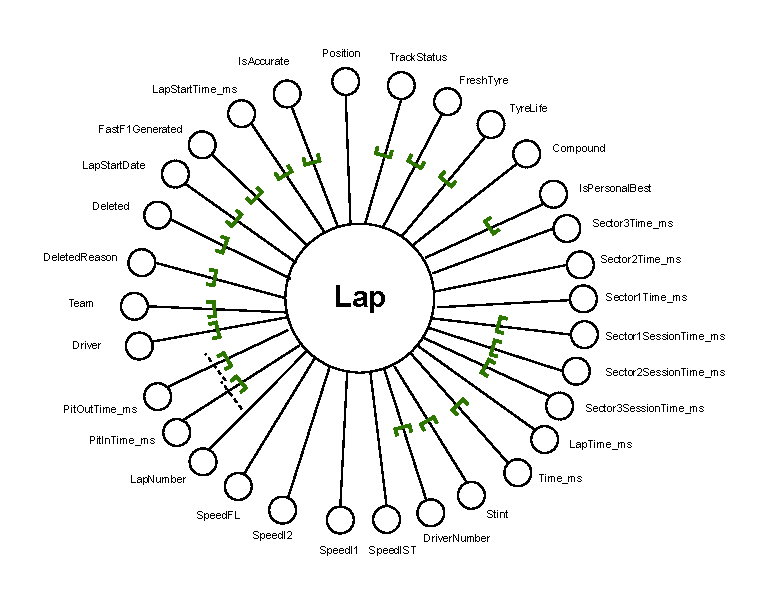
\includegraphics[
			width=\linewidth,
			trim=1.0cm 1.0cm 1.0cm 1.0cm,
			clip
			]{figures/lap_focus1.pdf}
			\caption{Pruning decisions}
			\label{fig:lap-pruning-editing-summary}
		\end{subfigure}
		\hfill
		\begin{subfigure}{0.495\linewidth}
			\centering
			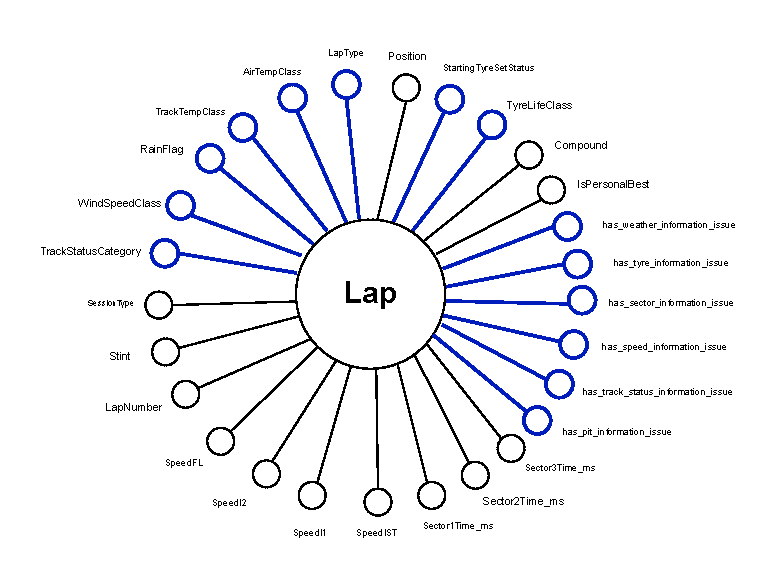
\includegraphics[
			width=\linewidth,
			trim=1.0cm 1.0cm 1.0cm 1.0cm,
			clip
			]{figures/lap_focus2.pdf}
			\caption{Derived-attribute decisions}
			\label{fig:lap-derived-editing-summary}
		\end{subfigure}
		
		\caption{Compact view of pruning and derived-attribute decisions for the Lap Performance fact.}
		\label{fig:lap-node-editing-summary}
	\end{figure}
	
	\begin{table}[H]
		\centering
		\small
		\caption{Representative pruning decisions for the \texttt{lap} node.}
		\label{tab:lap-pruning-representative}
		\renewcommand{\arraystretch}{1.15}
		\begin{tabularx}{\linewidth}{
				>{\raggedright\arraybackslash}p{3.6cm}
				>{\raggedright\arraybackslash}p{4.6cm}
				>{\raggedright\arraybackslash}X
			}
			\toprule
			\textbf{Pruned attribute}
			& \textbf{Attributes}
			& \textbf{Motivation} \\
			\midrule
			
			Session-timeline timestamps
			& \texttt{time\_ms}, \texttt{lap\_start\_time\_ms}, \texttt{lap\_start\_date}, \texttt{sector1\_session\_time\_ms}, \texttt{sector2\_session\_time\_ms}, \texttt{sector3\_session\_time\_ms}
			& These attributes represent absolute or session-relative passage times. The analysis does not require the exact time at which the driver crossed a lap or sector point. \\
			
			
			\midrule
			
			Redundant driver and team descriptors
			& \texttt{driver}, \texttt{driver\_number}, \texttt{team}
			& Driver and team are already represented through the shared Driver and Team dimensions. \\
			
			\midrule
			
			Raw pit timestamps
			& \texttt{pit\_in\_time\_ms}, \texttt{pit\_out\_time\_ms}
			& These timestamps do not measure the intrinsic competitive quality of a lap. \\
			
			\midrule
			
			Raw tyre usage attributes
			& \texttt{fresh\_tyre}, \texttt{tyre\_life}, \texttt{stint}
			& In their raw form, these attributes are too detailed for the tyre-related analysis. \\
			
			\midrule
			
			Source and quality-control attributes
			& \texttt{deleted}, \texttt{deleted\_reason}, \texttt{fastf1\_generated}, \texttt{is\_accurate}, \texttt{is\_personal\_best}
			& These attributes are useful for validation, cleaning, traceability, or raw source interpretation, but they are not final analytical dimensions. \\
	
				
			\midrule
			
			Raw track-status value
			& \texttt{track\_status}
			& The raw value is not sufficiently clear as an analytical category. \\
			
			\bottomrule
		\end{tabularx}
	\end{table}
	
	{\footnotesize
		\renewcommand{\arraystretch}{1.15}
		
		\begin{longtable}{
				>{\raggedright\arraybackslash}p{3.2cm}
				>{\raggedright\arraybackslash}p{3.0cm}
				>{\raggedright\arraybackslash}p{2.8cm}
				>{\raggedright\arraybackslash}p{6.5cm}
			}
			\caption{Representative derived attributes for the Lap Performance fact.}
			\label{tab:lap-derived-representative} \\
			
			\toprule
			\textbf{Derived attribute}
			& \textbf{Derived from}
			& \textbf{Categorical values}
			& \textbf{Motivation} \\
			\midrule
			\endfirsthead
			
			\toprule
			\textbf{Derived attribute}
			& \textbf{Derived from}
			& \textbf{Categorical values}
			& \textbf{Motivation} \\
			\midrule
			\endhead
			
			\midrule
			\multicolumn{4}{r}{\emph{Continued on next page}} \\
			\endfoot
			
			\bottomrule
			\endlastfoot
			
			\texttt{lap\_type}
			& \texttt{pit\_in\_time\_ms}, \texttt{pit\_out\_time\_ms}
			& Normal lap; In-lap; Out-lap
			& Distinguishes clean laps from laps affected by pit entry or pit exit. \\
			
			\midrule
			
			\texttt{tyre\_life\_class}
			& \texttt{tyre\_life}
			& Low; Medium; High
			& Groups the numerical tyre-life value into meaningful tyre-age categories. \\
			
			\midrule
			
			{\scriptsize\texttt{starting\_tyre\_set\_status}}
			& \texttt{fresh\_tyre}
			& New; Used
			& Describes the tyre set condition at the beginning of the stint. \\
			
			\midrule
			
			{\scriptsize\texttt{air\_temp\_class}, \texttt{track\_temp\_class}, \texttt{wind\_speed\_class}}
			& \texttt{weather.air\_temp}, \texttt{weather.track\_temp}, \texttt{weather.wind\_speed}
			& Low; Medium; High
			& Transform continuous weather values into categorical classes aligned with the lap interval. \\
			
			\midrule
			
			\texttt{rain\_flag}
			& \texttt{weather.rainfall}
			& True; False
			& Indicates whether rainfall was detected for the weather context associated with the lap. \\
			
			\midrule
			
			{\scriptsize\texttt{track\_status\_category}}
			& Track-status records aligned to the lap interval
			& All clear; Yellow flag; Safety Car; Virtual Safety Car; Red flag
			& Converts time-dependent track-status information into a lap-level category. \\
			
			\midrule
			
			{\scriptsize Lap data-quality flags}
			& Data-cleaning outputs
			& True; False
			& Flags unreliable or incomplete information in the corresponding data area. \\
			
		\end{longtable}
	}
	
	\subsubsection{Session Result Editing}
	
	The \textit{Session Result} fact is rooted in the \texttt{result} relation. 
	This fact requires a specific treatment because the same table contains both qualifying-related and race-related information. 
	Qualifying attributes are meaningful only for qualifying sessions, while race attributes are meaningful only for race sessions.
	
	Table~\ref{tab:result-pruning-representative} reports the pruning decisions applied to the \texttt{result} node. 
	After pruning, several derived attributes are introduced to transform heterogeneous or textual information into cleaner analytical attributes. 
	Table~\ref{tab:result-derived-representative} reports the main derived attributes used in the edited \textit{Session Result} tree.
	
	\begin{figure}[H]
		\centering
		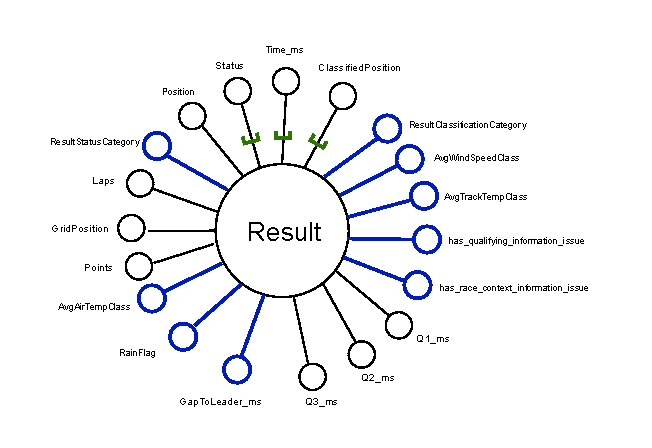
\includegraphics[width=0.70\linewidth]{figures/result_focus.pdf}
		\caption{Compact view of pruning and derived-attribute decisions for the Session Result fact.}
		\label{fig:result-node-editing-summary}
	\end{figure}
	
	\begin{table}[H]
		\centering
		\small
		\caption{Representative pruning decisions for the \texttt{result} node.}
		\label{tab:result-pruning-representative}
		\renewcommand{\arraystretch}{1.15}
		\begin{tabularx}{\linewidth}{
				>{\raggedright\arraybackslash}p{4.2cm}
				>{\raggedright\arraybackslash}X
			}
			\toprule
			\textbf{Attribute}
			& \textbf{Motivation} \\
			\midrule
			
			\texttt{classified\_position}
			& This attribute mixes numeric classifications and textual race-result codes. When it is numeric, it also repeats information already represented by \texttt{position}. \\
			
			\midrule
			
			\texttt{status}
			& This attribute is an open textual field with many sparse values. It is not suitable as a clean analytical category. \\
			
			\midrule
			
			\texttt{time\_ms}
			& In race sessions it may represent total time or gap from the winner, while in qualifying sessions it is normally not applicable. \\
			
			\bottomrule
		\end{tabularx}
	\end{table}
	
	{\footnotesize
		\renewcommand{\arraystretch}{1.15}
		
		\begin{longtable}{
				>{\raggedright\arraybackslash}p{3.4cm}
				>{\raggedright\arraybackslash}p{3.0cm}
				>{\raggedright\arraybackslash}p{3.8cm}
				>{\raggedright\arraybackslash}p{6.1cm}
			}
			\caption{Representative derived attributes for the Session Result fact.}
			\label{tab:result-derived-representative} \\
			
			\toprule
			\textbf{Derived attribute}
			& \textbf{Derived from}
			& \textbf{Values / interpretation}
			& \textbf{Motivation} \\
			\midrule
			\endfirsthead
			
			\toprule
			\textbf{Derived attribute}
			& \textbf{Derived from}
			& \textbf{Values / interpretation}
			& \textbf{Motivation} \\
			\midrule
			\endhead
			
			\midrule
			\multicolumn{4}{r}{\emph{Continued on next page}} \\
			\endfoot
			
			\bottomrule
			\endlastfoot
			
			{\scriptsize result\_classification\_category}
			& \texttt{classified\_position}
			& Classified; Retired; Disqualified; Excluded; Withdrawn; Not classified; Failed to qualify; Not applicable
			& Replaces a mixed numeric/textual field with a stable categorical description of the final classification state. \\
			
			\midrule
			
			{\scriptsize\texttt{result\_status\_category}}
			& \texttt{status}
			& Finished; Lapped; Accident; Collision; Power unit issue; Mechanical issue; Retired; Other; Not applicable
			& Groups raw textual race statuses into a limited set of interpretable result categories. \\
			
			\midrule
			
			\texttt{gap\_to\_leader\_ms}
			& \texttt{time\_ms}
			& Numerical value in milliseconds; \texttt{NULL} when not comparable
			& Converts the raw race time into a homogeneous measure representing the gap from the race leader. \\
			
			\midrule
			
			{\scriptsize\texttt{avg\_air\_temp\_class}, \texttt{avg\_track\_temp\_class}, \texttt{avg\_wind\_speed\_class}}
			& Aggregated session-level weather observations
			& Low; Medium; High
			& Summarizes continuous weather values at session level using categorical classes coherent with the result grain. \\
			
			\midrule
			
			\texttt{rain\_flag}
			& Session-level \texttt{weather.rainfall}
			& True; False
			& Indicates whether rainfall occurred during the session. \\
			
			\midrule
			
			{\scriptsize Result data-quality flags}
			& Data-cleaning outputs
			& True; False
			& Flags unreliable or incomplete information in the corresponding result data area. \\
			
		\end{longtable}
	}
	
	
	\subsection{Dimensions, Measures, and Aggregation Semantics}
	
	After the editing of the attribute trees, the remaining attributes are mapped into dimensions and measures. 
	Direct dimensions are obtained from explicit nodes or branches of the edited attribute tree, while measures correspond to numerical attributes analysed at the grain of the fact.
	
	Some final dimensions are not represented by a single node. 
	They are created by grouping related attributes that share the same analytical meaning. 
	In this project, two cases are distinguished: contextual or composite dimensions, which group related descriptive attributes, and junk dimensions, which group low-cardinality quality flags used to support filtering in OLAP analysis.
	
	\begin{table}[H]
		\centering
		\footnotesize
		\caption{Legend for dimensional mapping diagrams.}
		\label{tab:dimensional-mapping-legend}
		\renewcommand{\arraystretch}{1.25}
		\setlength{\tabcolsep}{8pt}
		\begin{tabular}{@{}c l c l@{}}
			\toprule
			\legendbox{directdimensioncolor} 
			& Direct dimension
			& \legendbox{measurecolor} 
			& Measure \\
			
			\addlinespace[0.15cm]
			
			\outlinedlegendbox{contextualboxcolor}{dashed} 
			& Contextual/composite dimension
			& \outlinedlegendbox{junkboxcolor}{densely dotted} 
			& Junk dimension \\
			\bottomrule
		\end{tabular}
	\end{table}
	
	\subsubsection{Lap Performance Dimensional Mapping}
	
	\begin{figure}[H]
		\centering
		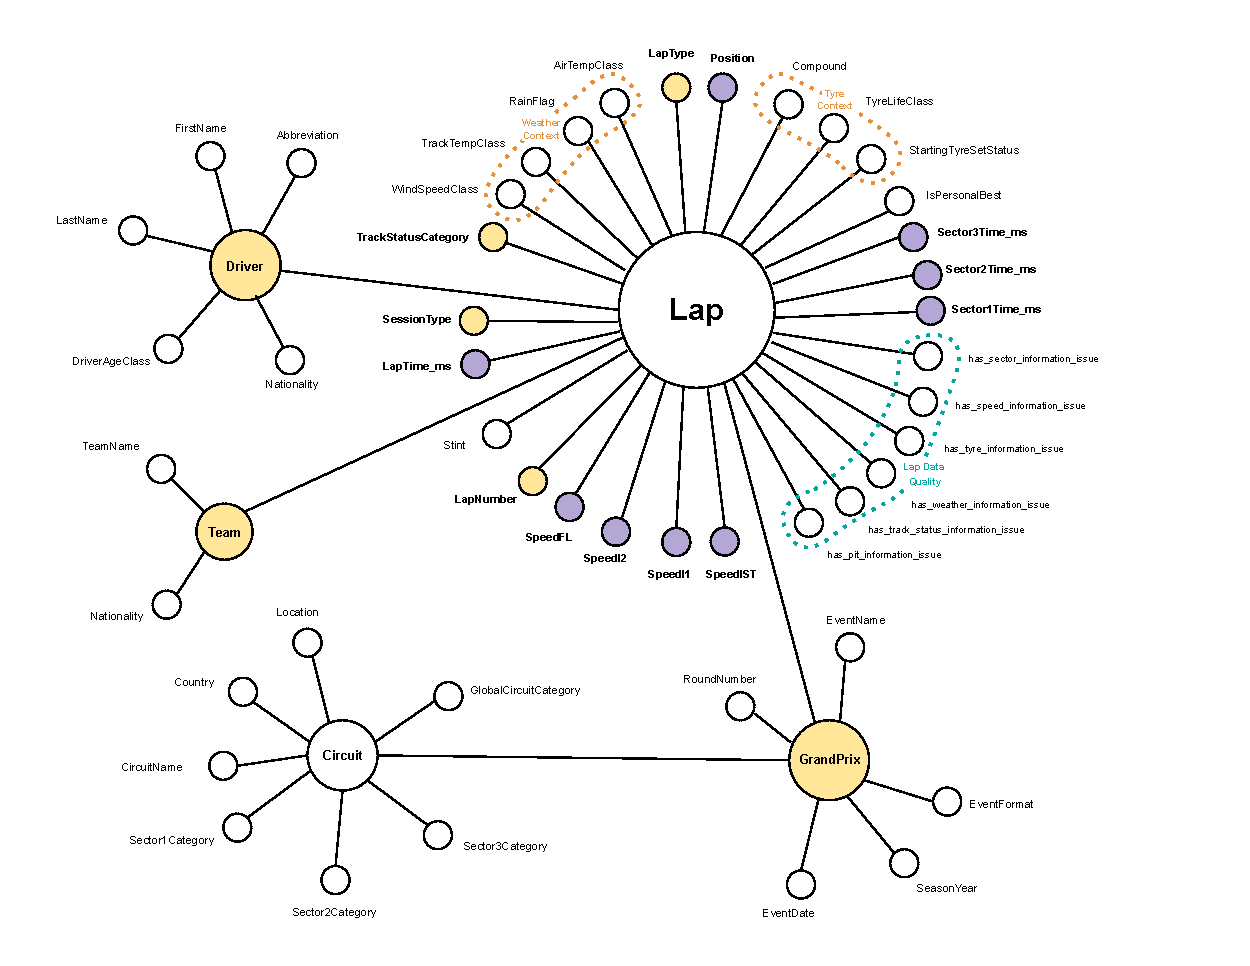
\includegraphics[width=1\linewidth]{figures/lap_final.pdf}
		\caption{Dimensional mapping for the Lap Performance fact.}
		\label{fig:lap-dimensional-mapping}
	\end{figure}
	
	\subsubsection{Lap Performance Measure Glossary}
	
	\begin{table}[H]
		\centering
		\small
		\caption{Measure glossary for the Lap Performance fact.}
		\label{tab:lap-performance-measure-glossary}
		\renewcommand{\arraystretch}{1.15}
		\begin{tabularx}{\linewidth}{
				>{\raggedright\arraybackslash}p{3.8cm}
				>{\raggedright\arraybackslash}X
				>{\raggedright\arraybackslash}p{4.2cm}
			}
			\toprule
			\textbf{Measure}
			& \textbf{Meaning}
			& \textbf{Aggregation semantics} \\
			\midrule
			
			\texttt{lap\_time\_ms}
			& Total lap duration in milliseconds.
			& \texttt{AVG}, \texttt{MIN}, \texttt{MAX}. Not additive. \\
			
			\midrule
			
			\texttt{sector1\_time\_ms}, \texttt{sector2\_time\_ms}, \texttt{sector3\_time\_ms}
			& Time spent in each circuit sector.
			& \texttt{AVG}, \texttt{MIN}, \texttt{MAX}. Not additive across laps. \\
			
			\midrule
			
			\texttt{speed\_i1}, \texttt{speed\_i2}, \texttt{speed\_fl}, \texttt{speed\_st}
			& Speed measurements recorded at intermediate points, finish line, and speed trap.
			& \texttt{AVG}, \texttt{MIN}, \texttt{MAX}. \\
			
			\midrule
			
			\texttt{position}
			& Driver position during the lap.
			& \texttt{MIN}, \texttt{MAX}; \texttt{AVG} only with caution. Not additive. \\
			
			\midrule
			
			\texttt{lap\_number}
			& Lap ordinal number within the session.
			& Used mainly for filtering or ordering; \texttt{MAX} can indicate the last observed lap. \\
			
			\midrule
			
			\texttt{lap\_count}
			& Number of lap records.
			& \texttt{COUNT}. Useful for counting analysed laps. \\
			
			\bottomrule
		\end{tabularx}
	\end{table}
	
	\subsubsection{Session Result Dimensional Mapping}
	
	\begin{figure}[H]
		\centering
		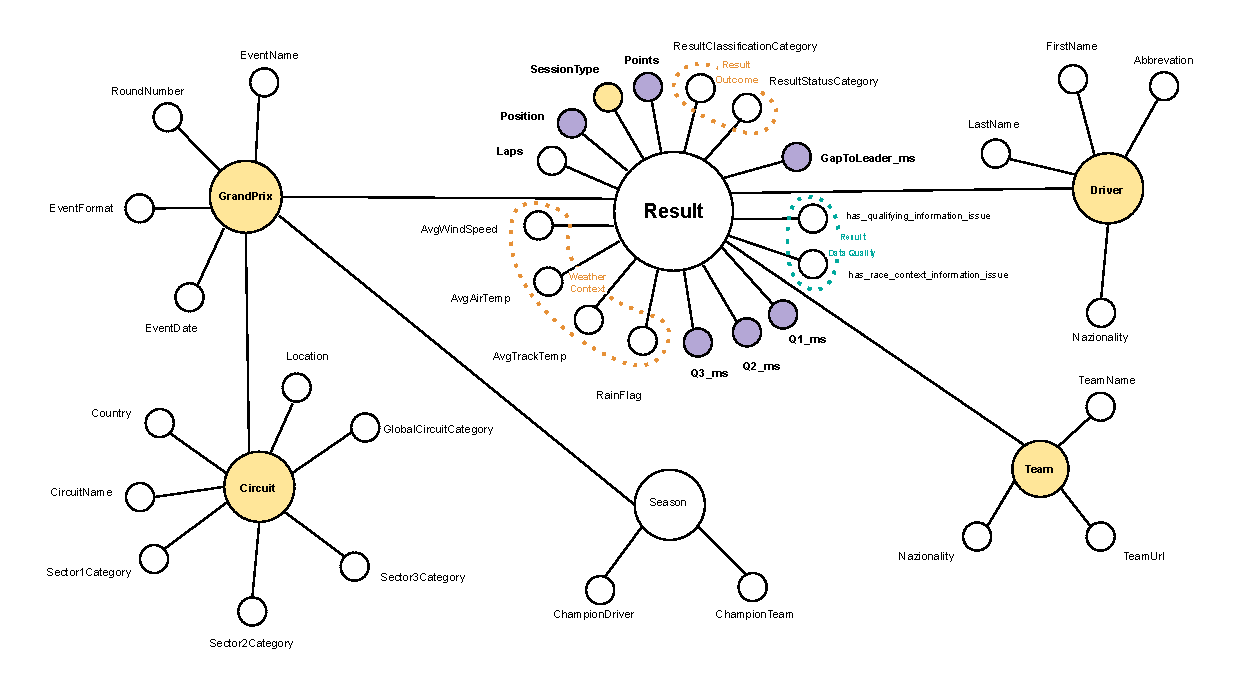
\includegraphics[width=1\linewidth]{figures/result_final.pdf}
		\caption{Dimensional mapping for the Session Result fact.}
		\label{fig:result-dimensional-mapping}
	\end{figure}
	
	\subsubsection{Session Result Measure Glossary}
	
	\begin{table}[H]
		\centering
		\small
		\caption{Measure glossary for the Session Result fact.}
		\label{tab:session-result-measure-glossary}
		\renewcommand{\arraystretch}{1.15}
		\begin{tabularx}{\linewidth}{
				>{\raggedright\arraybackslash}p{3.8cm}
				>{\raggedright\arraybackslash}X
				>{\raggedright\arraybackslash}p{4.2cm}
			}
			\toprule
			\textbf{Measure}
			& \textbf{Meaning}
			& \textbf{Aggregation semantics} \\
			\midrule
			
			\texttt{position}
			& Final position of the driver in the session result.
			& \texttt{MIN}, \texttt{MAX}; \texttt{AVG} only with caution. Not additive. \\
			
			\midrule
			
			\texttt{grid\_position}
			& Starting grid position, mainly meaningful for race sessions.
			& \texttt{MIN}, \texttt{MAX}; \texttt{AVG} only with caution. Not additive. \\
			
			\midrule
			
			\texttt{points}
			& Championship points obtained by the driver in the session.
			& \texttt{SUM}, \texttt{AVG}, \texttt{MAX}. Additive across drivers, teams, and races. \\
			
			\midrule
			
			\texttt{laps}
			& Number of completed laps in the session result.
			& \texttt{SUM}, \texttt{AVG}, \texttt{MAX}. Additive when counting completed laps. \\
			
			\midrule
			
			\texttt{q1\_ms}, \texttt{q2\_ms}, \texttt{q3\_ms}
			& Qualifying times recorded in each qualifying segment.
			& \texttt{AVG}, \texttt{MIN}, \texttt{MAX}. Not additive. \\
			
			\midrule
			
			\texttt{gap\_to\_leader\_ms}
			& Time gap from the session or race leader, when comparable.
			& \texttt{AVG}, \texttt{MIN}, \texttt{MAX}. Not additive. \\
			
			\midrule
			
			\texttt{result\_count}
			& Number of session-result records.
			& \texttt{COUNT}. Useful for counting analysed results. \\
			
			\bottomrule
		\end{tabularx}
	\end{table}
	
	\newpage
	\subsection{Final DFM Fact Schemas}
	
	The conceptual design phase ends with the definition of the two final DFM fact schemas. 
	These schemas summarize the facts, dimensions, measures, and hierarchies obtained from the edited attribute trees.
	
	\begin{figure}[H]
		\centering
		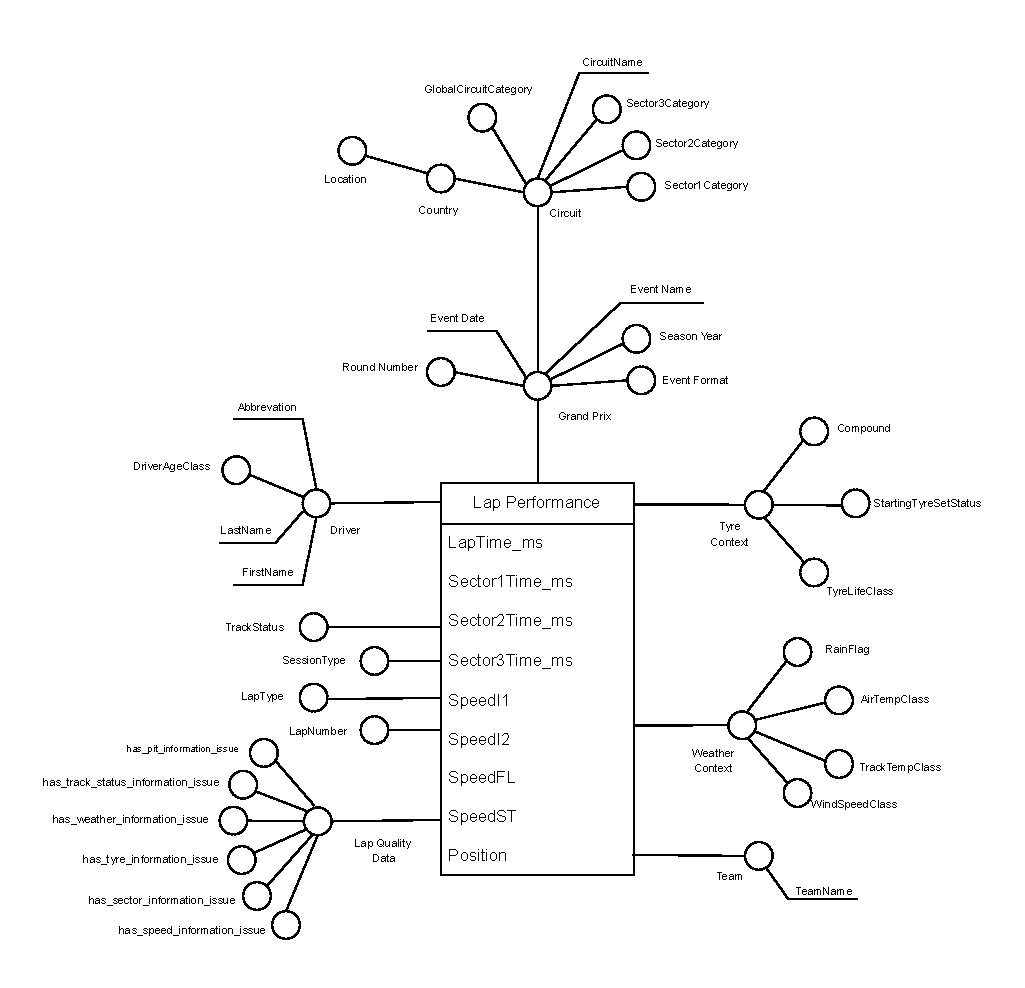
\includegraphics[width=0.65\linewidth]{figures/lap_fact_schema.pdf}
		\caption{Final DFM fact schema for the Lap Performance fact.}
		\label{fig:dfm-lap-performance}
	\end{figure}
	
	\begin{figure}[H]
		\centering
		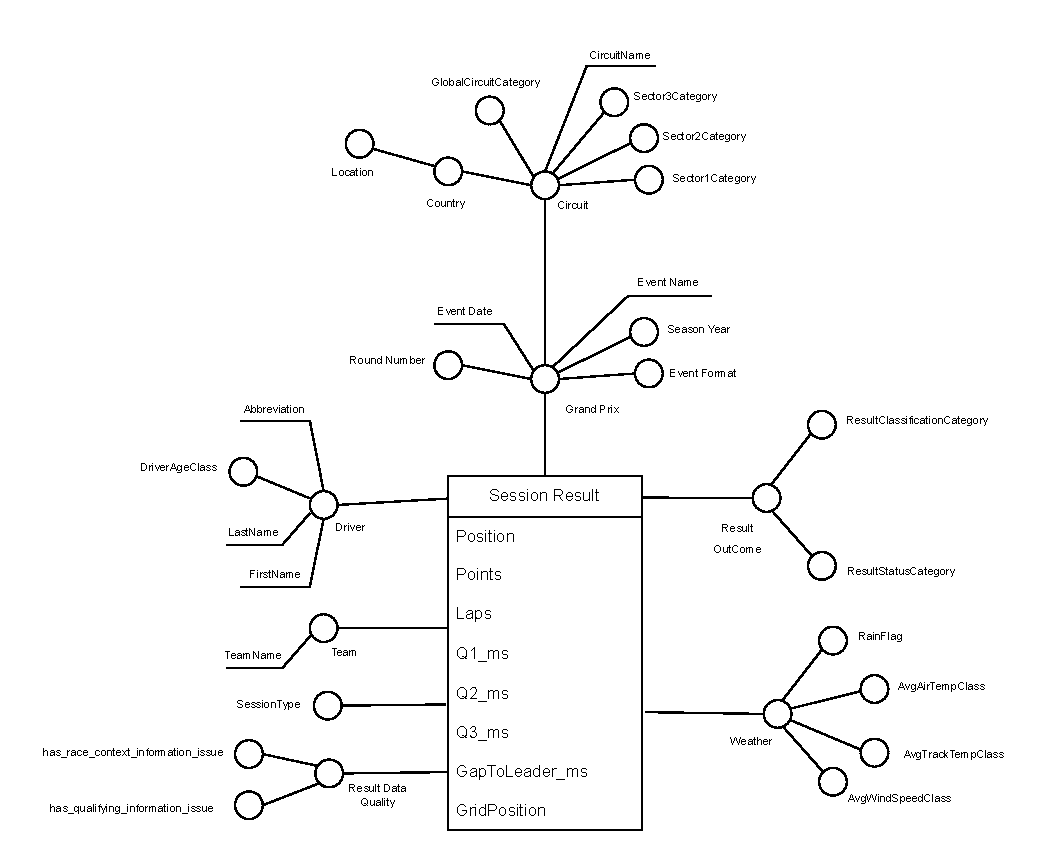
\includegraphics[width=0.65\linewidth]{figures/result_fact_schema.pdf}
		\caption{Final DFM fact schema for the Session Result fact.}
		\label{fig:dfm-session-result}
	\end{figure}
	
	
	
	\section{Logical Design: Star Schema}
	

	
	The logical design translates the two conceptual DFM fact schemas into relational star schemas inside the \texttt{warehouse} schema. 
	At this level, conceptual facts and dimensions are converted into implementation-oriented tables using the \texttt{snake\_case} naming convention adopted in the database.
	
	The two fact tables preserve the analytical grains defined during conceptual design. 
	Shared dimensions are implemented only once and connected to both facts, allowing integrated analysis across lap-level performance and session-level results.
	
	\vspace{2em}
	\subsection{Integrated Logical Star Schema}
	
	For readability, the main report shows a compact logical star schema with table names only. 
	The complete star schema diagrams with all attributes are reported in Appendix~\ref{appendix:star-schema-details}.
	
	\vspace{2em}
	\begin{figure}[H]
		\centering
		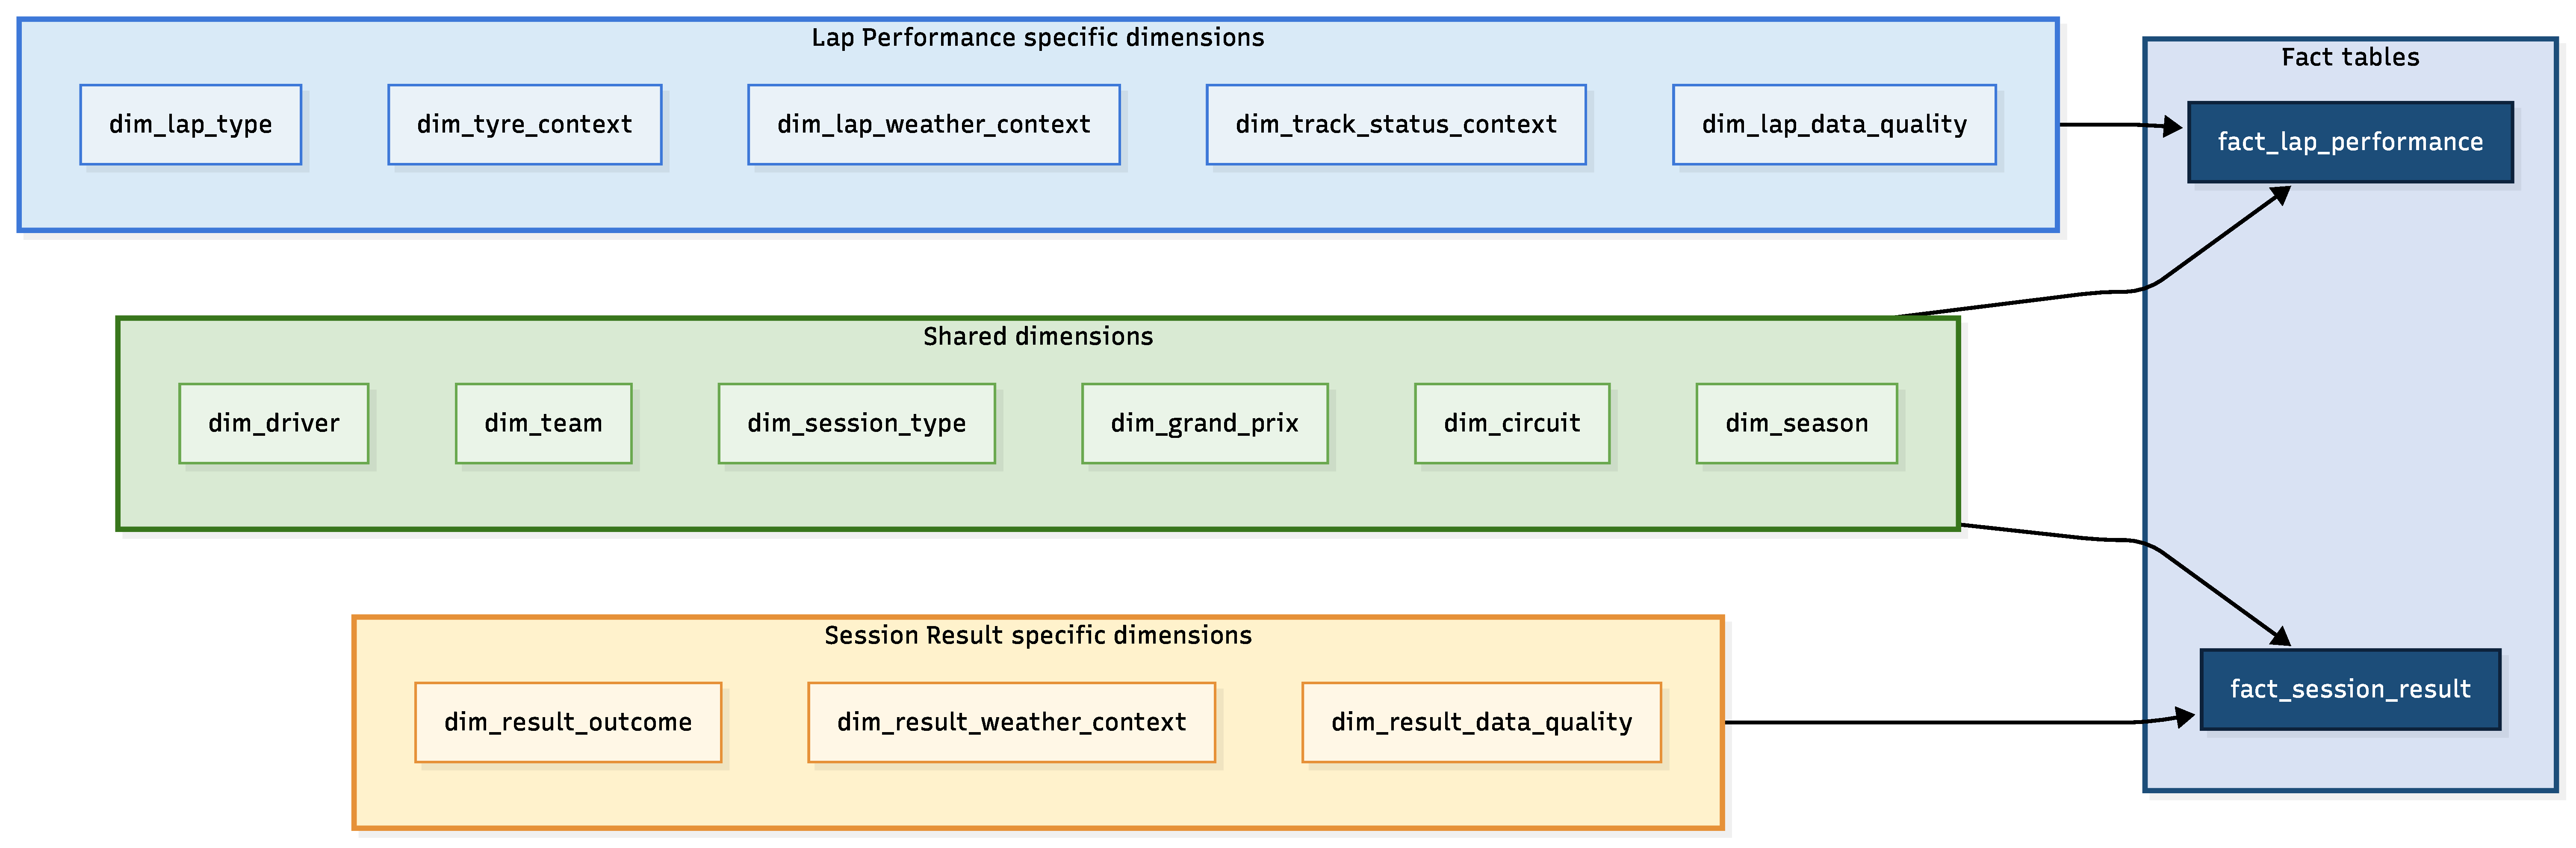
\includegraphics[width=1\linewidth]{figures/integrated_star_schema.pdf}
		\caption{Integrated logical star schema with shared and fact-specific dimensions.}
		\label{fig:integrated-star-schema}
	\end{figure}
	
	\vspace{2em}
	\begin{table}[H]
		\centering
		\caption{Logical star schema summary.}
		\label{tab:star-summary}
		\begin{tabularx}{\linewidth}{p{4.5cm}X}
			\toprule
			\textbf{Table type} & \textbf{Tables} \\
			\midrule
			Fact tables 
			& \texttt{fact\_lap\_performance}, \texttt{fact\_session\_result} \\
			\midrule
			Shared dimensions 
			& \texttt{dim\_driver}, \texttt{dim\_team}, \texttt{dim\_grand\_prix}, \texttt{dim\_circuit}, \texttt{dim\_season}, \texttt{dim\_session\_type} \\
			\midrule
			Lap-specific dimensions 
			& \texttt{dim\_tyre\_context}, \texttt{dim\_weather\_context}, \texttt{dim\_track\_status}, \texttt{dim\_lap\_type}, \texttt{dim\_lap\_data\_quality} \\
			\midrule
			Result-specific dimensions 
			& \texttt{dim\_result\_status}, \texttt{dim\_result\_data\_quality} \\
			\bottomrule
		\end{tabularx}
	\end{table}

	
	\newpage
	\section{Conclusion}
	
	This report documented the construction of a Formula 1 Data Warehouse starting from heterogeneous API-based and manually curated sources. 
	The raw data were first re-engineered into a reconciled PostgreSQL schema, then assessed through data quality checks, missing-value interpretation, outlier detection, and conservative cleaning rules.
	
	The cleaned layer was used to design two complementary analytical facts: \textit{Lap Performance}, focused on lap-level performance, and \textit{Session Result}, focused on driver outcomes at session level. 
	The conceptual design produced two DFM fact schemas, while the logical design translated them into an integrated star schema with shared dimensions and fact-specific analytical contexts.
	
	The resulting warehouse provides a structured and OLAP-ready basis for the next phase of the project, where the star schema can be used in Tableau to analyse performance differences across seasons, teams, drivers, sessions, circuits, tyres, and race conditions.
	
   % TODO generate dimensionbs

	\section{Repository}
	\label{sec:repository-material}
	
	Full code, detailed DQA outputs, cleaning logs, rejected rows, and full schema files are available in the project repository:
	\url{https://github.com/GiuseppeRudi/groundeffect-dw}
	

	
	\begin{thebibliography}{9}
		
		\bibitem{f1calendars}
		Formula 1 Official Website.
		\textit{Formula 1 Calendars for the 2021 and 2022 seasons}.
		Available at:
		\url{https://www.formula1.com/en/racing/2021},
		\url{https://www.formula1.com/en/racing/2022}
		
		\bibitem{f1standings}
		Formula 1 Official Website.
		\textit{Formula 1 Drivers' and Constructors' Standings for the 2021 and 2022 seasons}.
		Available at:
		\url{https://www.formula1.com/en/results/2021/drivers},
		\url{https://www.formula1.com/en/results/2022/drivers},
		\url{https://www.formula1.com/en/results/2021/team},
		\url{https://www.formula1.com/en/results/2022/team}
		
		\bibitem{formulaTimerCircuits}
		Formula Timer.
		\textit{Formula 1 Circuit Information}.
		Available at:
		\url{https://formula-timer.com/circuit}
		
	\end{thebibliography}

	

	

	\newpage
	\appendix
	
	
	
	\section{Additional Re-engineering Material}
	\label{appendix:reengineering-material}
	

	\vspace{3em}
	\subsection{Complete Raw API Structures}
	\label{appendix:raw-api-structures}
	
	
	\vspace{5em}
	\begin{figure}[H]
		\centering
		
\includegraphics[width=0.90\linewidth,height=0.88\textheight,keepaspectratio]{figures/raw_tables.pdf}
		\caption{Complete raw API structures with original attributes.}
		\label{fig:appendix-raw-api-structures}
	\end{figure}
	
	\newpage
	
	\vspace{3em}
	\subsection{Complete Logical Schema}
	\label{appendix:logical-schema}
	
	
	\vspace{7em}
	\begin{figure}[H]
		\centering
		
\includegraphics[width=1\linewidth]{figures/logical_schema.pdf}
		\caption{Complete logical schema of the reconciled database.}
		\label{fig:appendix-logical-schema}
	\end{figure}
	
	\newpage

	\section{Additional Data Quality Material}
	\label{appendix:data-quality-details}
	
	\vspace{3em}
	\subsection{Detailed DQA Rules}
	
	\vspace{1.5em}
	\label{appendix:dqa-rules}
	

	
	\begin{longtable}{
			>{\raggedright\arraybackslash}p{2.8cm}
			>{\raggedright\arraybackslash}p{4.6cm}
			>{\raggedright\arraybackslash}p{7.4cm}
		}
		\caption{Summary of additional DQA rules by quality dimension.}
		\label{tab:appendix-dqa-rules} \\
		\toprule
		\textbf{Dimension}
		& \textbf{Rule families}
		& \textbf{Applied checks} \\
		\midrule
		\endfirsthead
		
		\toprule
		\textbf{Dimension}
		& \textbf{Rule families}
		& \textbf{Examples} \\
		\midrule
		\endhead
		
		\bottomrule
		\endfoot
		
		Completeness
		& Required identifiers, foreign keys, and core analytical attributes.
		& season\_year; grand\_prix\_id; session\_id; driver\_id; team\_id; lap\_number; time\_ms. \\
		
		\midrule
		
		Uniqueness
		& Primary-key and natural-key uniqueness.
		& season\_year; grand\_prix\_id; season\_year + round\_number; grand\_prix\_id + session\_type; session\_id + time\_ms. \\
		
		\midrule
		
		Validity
		& Allowed domains, formats, and numerical ranges.
		& event\_format; session\_type; compound; track\_status; lap\_number $> 0$; points $\geq 0$; valid URLs. \\
		
		\midrule
		
		Consistency
		& Coherence between related values.
		& Season dates order; event date coherent with season; session date coherent with Grand Prix date; sector-time sum coherent with lap\_time\_ms; track-status code coherent with message. \\
		
		\midrule
		
		Accuracy
		& Broad plausibility checks on values without a direct external truth source.
		& Driver age; air temperature; track temperature; pressure; track-air temperature difference. \\
		
		\midrule
		
		Referential Integrity
		& Foreign-key existence between child and parent tables.
		& grand\_prix $\rightarrow$ season; grand\_prix $\rightarrow$ circuit; session $\rightarrow$ grand\_prix; lap/result $\rightarrow$ session, driver, team. \\
		
	\end{longtable}
	
	\noindent\footnotesize{\textit{Note:} Timeliness is excluded because the project uses historical seasons; temporal checks are treated as consistency rules.}
	
	\newpage
	
	\subsection{Lap-table Missing Rules}
	\label{appendix:missing-rules}
	
	The main report reports only the pit-related cases and the missing \texttt{lap\_time\_ms} rule.
	The remaining lap-level rules are reported here because they affect more specific analytical areas.
	
	\begin{table}[H]
		\centering
		\small
		\caption{Sector-time missing-value rules for the \texttt{lap} table.}
		\label{tab:appendix-lap-sector-missing-rules}
		\begin{tabularx}{\linewidth}{p{4cm}p{3.2cm}p{3.2cm}X}
			\toprule
			\textbf{Condition}
			& \textbf{Missing attribute}
			& \textbf{Missing class}
			& \textbf{Information area} \\
			\midrule
			

			\texttt{pit\_in\_time\_ms} is present.
			& \texttt{sector3\_time\_ms}
			& \texttt{EXPLAINED NULL}
			& \texttt{SECTOR INFORMATION} \\
			
			\midrule
			
			No direct sector-specific explanation is available.
			& Any missing sector time
			& \texttt{SUSPICIOUS NULL}
			& \texttt{SECTOR INFORMATION} \\
			
			\bottomrule
		\end{tabularx}

		
	\end{table}
	
	\begin{table}[H]
		\centering
		\small
		\caption{Speed missing-value rules for the \texttt{lap} table.}
		\label{tab:appendix-lap-speed-missing-rules}
		\begin{tabularx}{\linewidth}{p{4cm}p{3.2cm}p{3.2cm}X}
			\toprule
			\textbf{Condition}
			& \textbf{Missing attribute}
			& \textbf{Missing class}
			& \textbf{Information area} \\
			\midrule
			

			\texttt{pit\_in\_time\_ms} is present.
			& \texttt{speed\_i1}, \texttt{speed\_fl}, or \texttt{speed\_st}
			& \texttt{EXPLAINED NULL}
			& \texttt{SPEED INFORMATION} \\
			
			\midrule
			
			\texttt{pit\_out\_time\_ms} is present.
			& \texttt{speed\_i1}, \texttt{speed\_fl}, or \texttt{speed\_st}
			& \texttt{EXPLAINED NULL}
			& \texttt{SPEED INFORMATION} \\
			
			\midrule
			
			Only pit information is available.
			& \texttt{speed\_i2}
			& \texttt{SUSPICIOUS NULL}
			& \texttt{SPEED INFORMATION} \\
			
			\midrule
			
			No pit-related explanation, not deleted, and accurate lap.
			& Any missing speed attribute
			& \texttt{SUSPICIOUS NULL}
			& \texttt{SPEED INFORMATION} \\
			
			\bottomrule
		\end{tabularx}
		
	\end{table}
	
	\begin{table}[H]
		\centering
		\small
		\caption{Tyre and compound missing-value rules for the \texttt{lap} table.}
		\label{tab:appendix-lap-tyre-missing-rules}
		\begin{tabularx}{\linewidth}{p{3.5cm}p{3.2cm}p{3.6cm}X}
			\toprule
			\textbf{Condition}
			& \textbf{Missing attribute}
			& \textbf{Missing class}
			& \textbf{Information area} \\
			\midrule
			

			Any lap
			& \texttt{compound}
			& \texttt{SUSPICIOUS NULL}
			& \texttt{TYRE INFORMATION} \\
			
			\midrule
			
			Any lap
			& \texttt{tyre\_life}
			& \texttt{SUSPICIOUS NULL}
			& \texttt{TYRE INFORMATION} \\
			
			\bottomrule
		\end{tabularx}

		
	\end{table}
	
	\begin{table}[H]
		\centering
		\small
		\caption{Track-status and weather-context missing-value rules for the \texttt{lap} table.}
		\label{tab:appendix-lap-context-missing-rules}
		\begin{tabularx}{\linewidth}{p{4cm}p{3.6cm}p{3.2cm}X}
			\toprule
			\textbf{Condition}
			& \textbf{Missing attribute}
			& \textbf{Missing class}
			& \textbf{Information area} \\
			\midrule
			

			Any lap
			& \texttt{track\_status}
			& \texttt{SUSPICIOUS NULL}
			& \texttt{TRACK STATUS INFORMATION} \\
			
			\midrule
			
			Future derived weather context is missing.
			& Weather-derived lap attribute
			& \texttt{SUSPICIOUS NULL}
			& \texttt{WEATHER INFORMATION} \\
			
			\bottomrule
		\end{tabularx}

		
	\end{table}


	\newpage
		
	\subsection{LLM-supported I/O}
	\label{appendix:llm-dqa-interpretation}
	
	\vspace{3em}
	
	\subsubsection*{Prompt provided to the LLM}
	
	\vspace{4em}
	
	\begin{lstlisting}
		
		
		You are an assistant supporting a Data Warehouse project about Formula 1 data.
		
		You receive only aggregated outputs from deterministic data quality analyses:
		- the general Data Quality Assessment,
		- the focused missing-values analysis,
		- the focused lap outlier detection.
		
		You do NOT have access to the database.
		You must NOT invent values, rules, or hidden causes.
		You must explain only what is supported by the provided scorecards, missing-value summaries, and outlier summaries.
		
		The DQA dimensions are:
		- Completeness
		- Uniqueness
		- Validity
		- Consistency
		- Accuracy/Plausibility
		- Timeliness
		- Referential Integrity
		
		Generate exactly these three Markdown sections:
		
		# Stakeholder Summary
		Write a clear, non-technical explanation of the general data quality situation.
		Mention the strongest and weakest tables if supported by the data.
		Include the focused missing-value and outlier signals when they materially change the interpretation.
		
		# Technical Summary
		Explain the main issues by table, quality dimension, missing information area, and outlier metric.
		Use precise language and avoid claiming that a value is wrong when it is only suspicious.
		
		# Suggested Cleaning Priorities
		Provide a prioritized list of next steps.
		The list must be framed as suggestions for human review, not automatic actions.
		
		Important rules:
		- Do not say that the LLM performed the official DQA.
		- Do not say that data were cleaned.
		- Do not recommend deleting records automatically.
		- Treat suspicious missing values and strong consensus outliers as human-review priorities, not proven errors.
		- Mention that the LLM output must be manually reviewed.
		- Keep the explanation useful for a final project report.
		
		Here is the aggregated complete data quality input:
		
		```json
		{{DATA_QUALITY_INPUT_JSON}}
		```
		
		
		
	\end{lstlisting}
	
	\newpage
	
	\vspace{2em}
	\subsubsection*{Compact Example of Generated Output}
	
	\vspace{2em}
	The following example shows the type of output generated by the LLM. 
	The content is intentionally shortened because LLM responses are not deterministic and can vary across executions. 
	The example is included only to document the expected structure of the response.
	
	\vspace{4em}
	\begin{lstlisting}
		
		
		# Stakeholder Summary
		
		The Formula One data warehouse shows a very high general quality level. 
		Most structural checks, such as uniqueness, validity, consistency, and referential integrity, report almost perfect scores.
		
		However, this does not mean that the data are free from quality issues. 
		The most relevant problems are concentrated in focused analyses: missing values in lap-level timing, sector, speed, and tyre information, and numerical outliers in lap and speed metrics.
		
		Overall, the warehouse is suitable for analysis, but some lap-level measures should be interpreted with quality flags or filtered when the analysis depends on the affected data area.
		
		# Technical Summary
		
		The general DQA mainly highlights small issues in the lap, result, and track_status tables. 
		The lap table contains most of the remaining validity warnings, while track_status shows a small uniqueness issue.
		
		The missing-value analysis shows that null values are not all equivalent. 
		Some are explained by the Formula One domain, while others are suspicious and require review. 
		The largest missing-value areas are speed information, sector information, and lap-time information.
		
		The outlier detection identifies several unusual values, especially for speed and lap-time metrics. 
		These values are not automatically considered errors, because unusual racing situations can naturally produce extreme observations.
		
		# Suggested Cleaning Priorities
		
		1. Review suspicious missing lap-time values before using lap time as a core measure.
		2. Check missing sector and speed information when the analysis depends on those metrics.
		3. Inspect strong consensus outliers in speed and lap-time metrics.
		4. Preserve uncertain records with quality flags when the issue cannot be corrected deterministically.
		5. Manually review all LLM suggestions before applying any cleaning decision.
		
		
	\end{lstlisting}
	
	
	\newpage


	\section{Additional DQA-driven Cleaning Rules}
	\label{appendix:dqa-cleaning-rules}
	
	\begin{longtable}{
			>{\centering\arraybackslash}m{2.6cm}
			>{\raggedright\arraybackslash}m{7.0cm}
			>{\raggedright\arraybackslash}m{5.3cm}
		}
		\caption{Additional grouped DQA-driven cleaning rules.}
		\label{tab:appendix-dqa-cleaning-rules} \\
		\toprule
		\textbf{Table}
		& \textbf{DQA issue}
		& \textbf{Cleaning action} \\
		\midrule
		\endfirsthead
		
		\toprule
		\textbf{Table}
		& \textbf{DQA issue}
		& \textbf{Cleaning action} \\
		\midrule
		\endhead
		
		\bottomrule
		\endfoot
		
		All tables
		& Primary-key violations, natural-key violations, or broken foreign-key references.
		& DROP ROW \\
		
		\midrule
		
		\multirow{2}{*}{season}
		& Missing structural key or season year outside the Formula 1 historical domain.
		& DROP ROW \\
		\cmidrule(l){2-3}
		
		& Invalid number of events or inconsistent season dates.
		& SET NULL \\
		
		\midrule
		
		\multirow{2}{*}{driver}
		& Missing required identification attributes.
		& DROP ROW \\
		\cmidrule(l){2-3}
		
		& Invalid abbreviation, URL, permanent number, or implausible birth-date-derived age.
		& SET NULL \\
		
		\midrule
		
		\multirow{2}{*}{team}
		& Missing required identification attributes.
		& DROP ROW \\
		\cmidrule(l){2-3}
		
		& Invalid team URL.
		& SET NULL \\
		
		\midrule
		
		\multirow{3}{*}{grand\_prix}
		& Missing structural attributes or invalid round number.
		& DROP ROW \\
		\cmidrule(l){2-3}
		
		& Invalid event format.
		& STANDARDIZE / DROP ROW \\
		\cmidrule(l){2-3}
		
		& Event date not coherent with the season year.
		& SET NULL \\
		
		\midrule
		
		\multirow{3}{*}{session}
		& Missing structural attributes.
		& DROP ROW \\
		\cmidrule(l){2-3}
		
		& Invalid session type.
		& STANDARDIZE / DROP ROW \\
		\cmidrule(l){2-3}
		
		& Session date not coherent with the Grand Prix date.
		& SET NULL \\
		
		\midrule
		
		\multirow{2}{*}{lap}
		& Sector-time sum not coherent with lap time.
		& ADD FLAG {\scriptsize(has\_sector\_information\_issue)} \\
		\cmidrule(l){2-3}
		
		& Unknown compound after deterministic standardization.
		& SET NULL + ADD FLAG {\scriptsize(has\_tyre\_information\_issue)} \\
		
		\midrule
		
		\multirow{2}{*}{weather}
		& Missing required attributes or invalid session-relative time.
		& DROP ROW \\
		\cmidrule(l){2-3}
		
		& Invalid weather range values or implausible track-air temperature relation.
		& SET NULL \\
		
		\midrule
		
		\multirow{4}{*}{track\_status}
		& Missing required attributes or invalid session-relative time.
		& DROP ROW \\
		\cmidrule(l){2-3}
		
		& Unknown status code.
		& DROP ROW \\
		\cmidrule(l){2-3}
		
		& Invalid status message with valid status code.
		& STANDARDIZE / SET NULL \\
		\cmidrule(l){2-3}
		
		& Status-code and message mismatch.
		& STANDARDIZE \\
		
	\end{longtable}
	
	
	
	\newpage
	

	\section{Additional Logical Star Schema Material}
	\label{appendix:star-schema-details}
	
	\vspace{2em}
	This appendix section can be used to report full-size versions of the star schema diagrams if the figures in the main report are simplified.
	
	\vspace{2em}
	\subsection{Full-size Lap Performance Star Schema}
	
	\begin{figure}[H]
		\centering
		 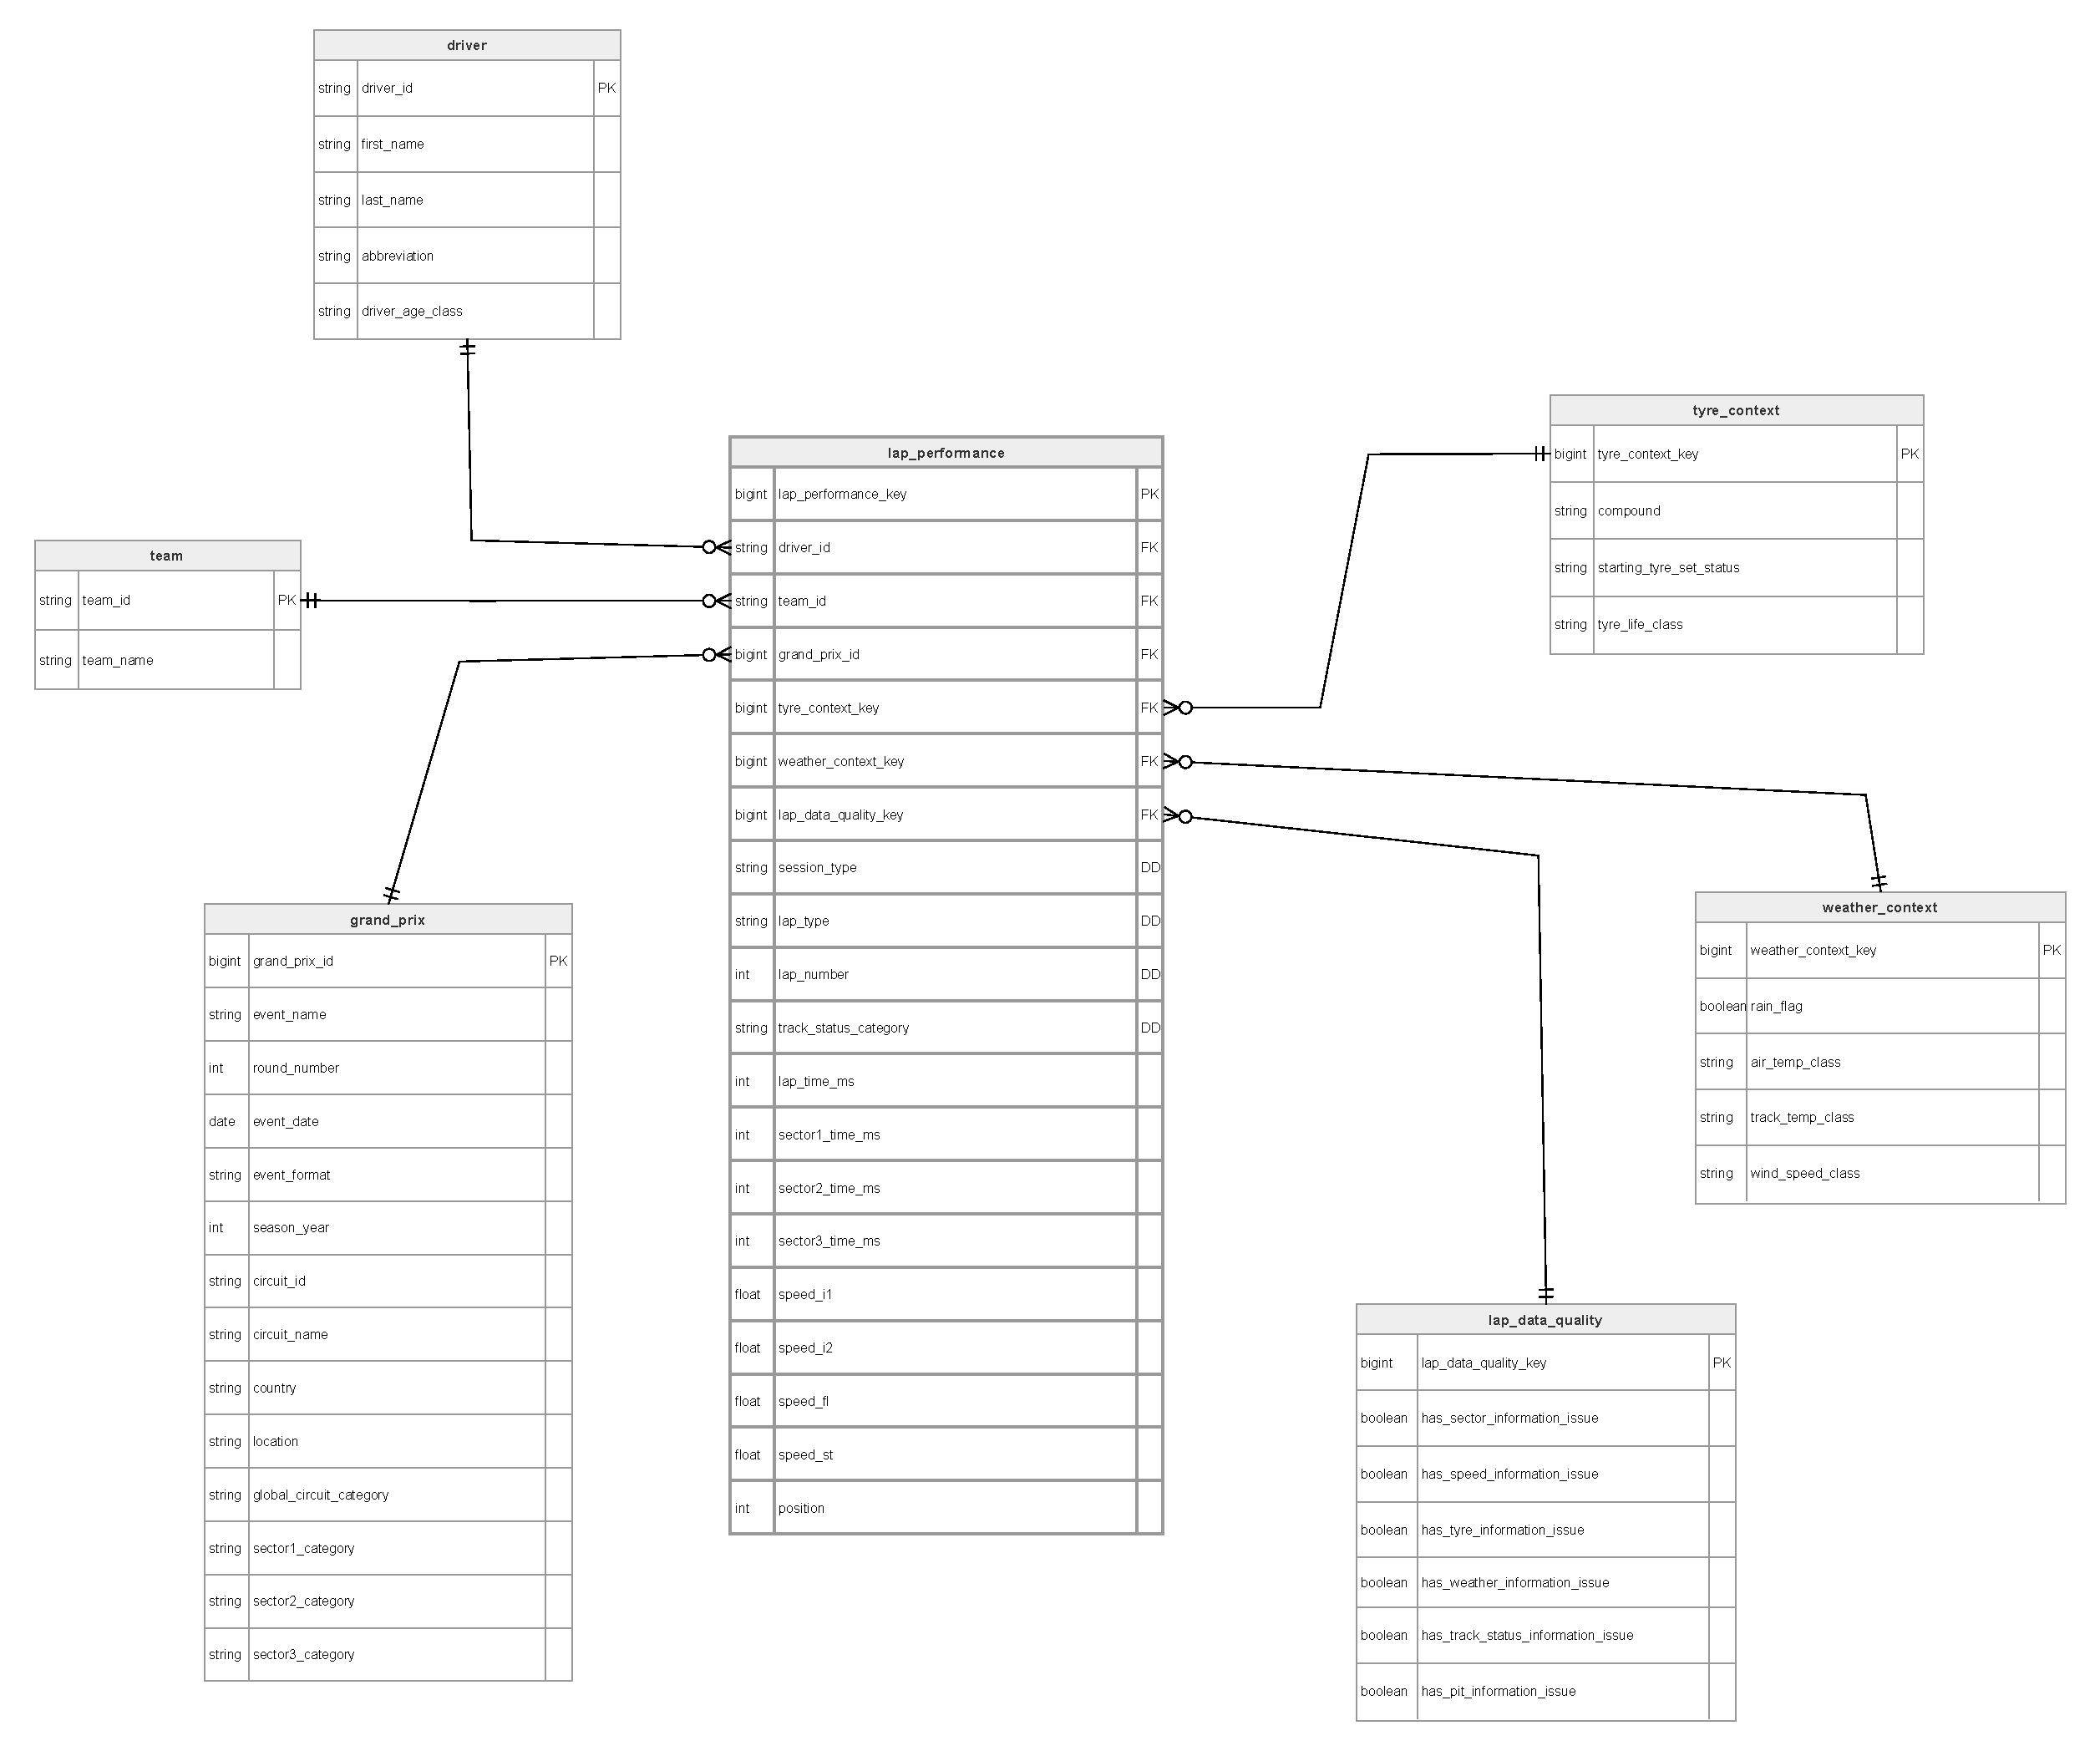
\includegraphics[width=1\linewidth,height=0.88\textheight,keepaspectratio]{figures/lap_star_schema.pdf}
		\caption{Full-size logical star schema for the Lap Performance fact.}
		\label{fig:appendix-star-lap}
	\end{figure}
	
	\subsection{Full-size Session Result Star Schema}
	
	\begin{figure}[H]
		\centering
		 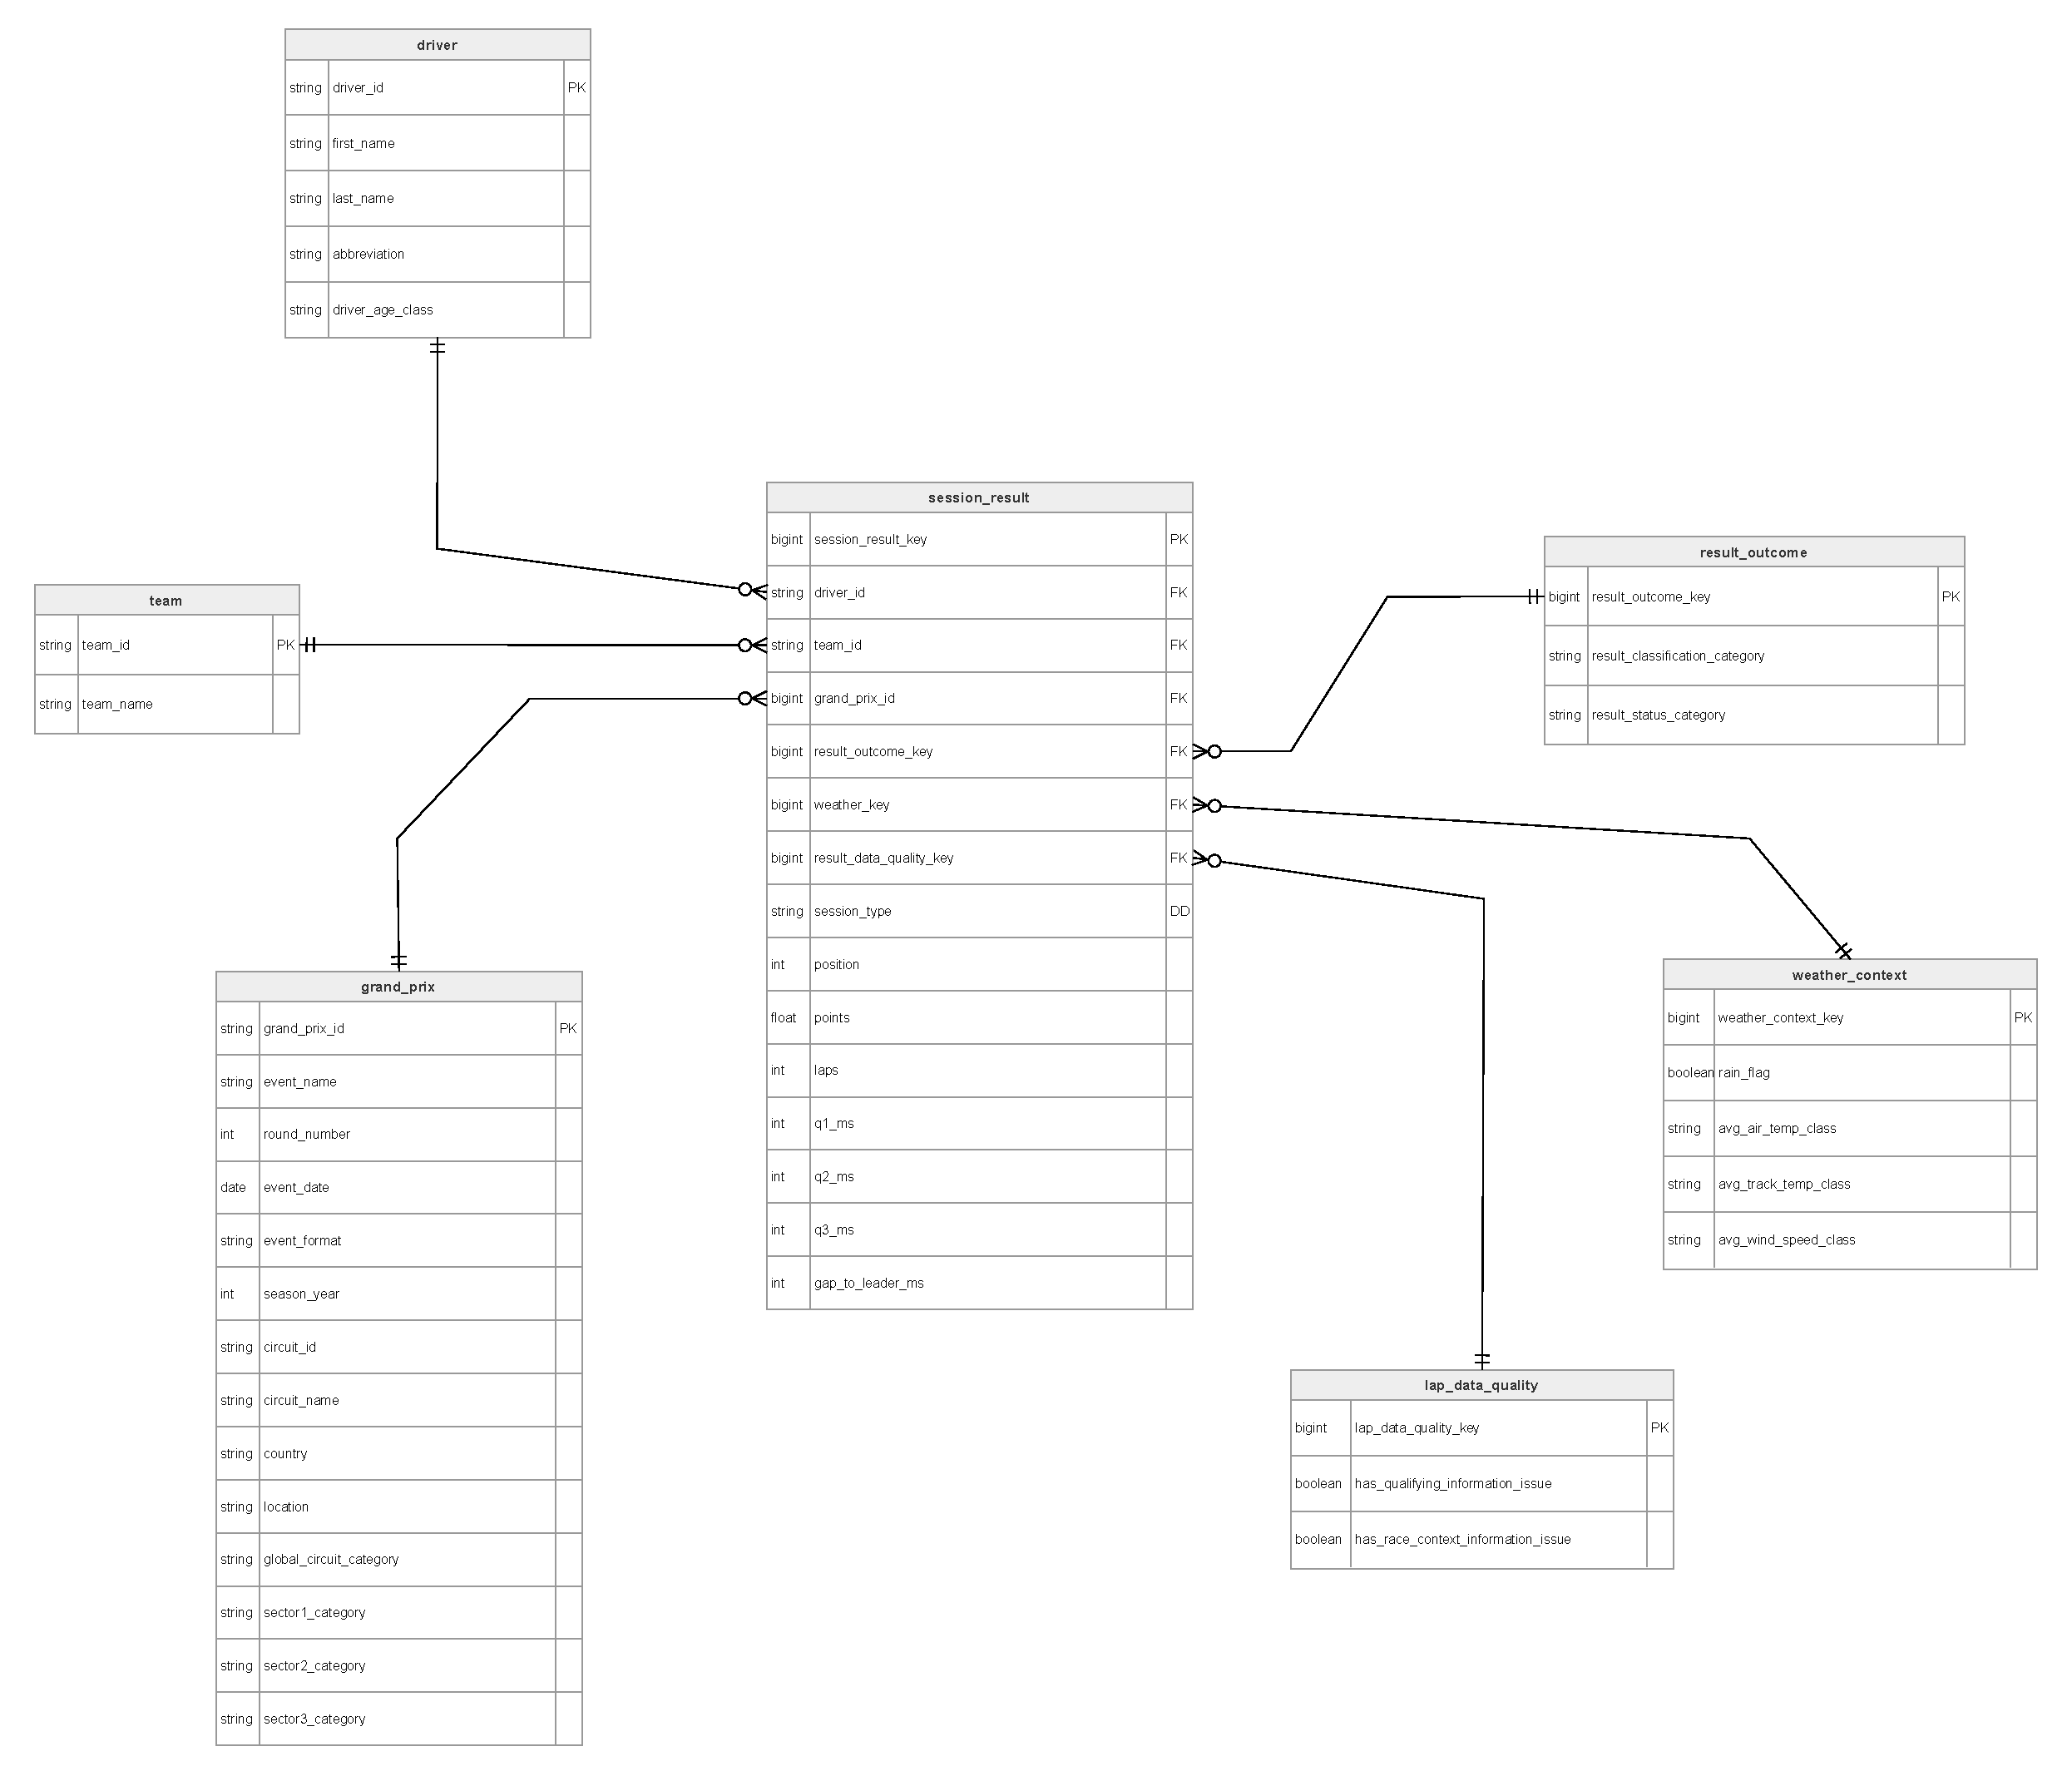
\includegraphics[width=1\linewidth,height=0.88\textheight,keepaspectratio]{figures/result_star_schema.pdf}
	
		\caption{Full-size logical star schema for the Session Result fact.}
		\label{fig:appendix-star-result}
	\end{figure}

	
	
\end{document}

